\chapter{Método Proposto}
\label{cap:materiais-metodo}
\phantom{0}

Este capítulo descreve o método proposto para segmentar os rins e tumores renais em TCs de pacientes doentes. A base de imagens usada para validar o método proposto é descrita na Seção~\ref{sec:conjunto-dados}. Inicialmente, foi realizada a etapa de pré-processamento em todos os volumes de TC da base de imagens, seguindo fluxos diferentes para os modelos de segmentação. Na segunda etapa, a segmentação inicial dos rins foi realizada usando o modelo ResUNet 2.5D e a segmentação inicial a candidatos de tumores renais foi realizado em duas subetapas: na primeira, os candidatos a tumores renais foram segmentados dentro da região renal usando o modelo DeepLabv3+ 2.5D; na segunda, foram segmentados dentro da região abdominal usando o modelo ResUNet 2.5D. Na terceira etapa, a reconstrução das regiões tumorais é realizada por meio da segmentação de candidatos a tumores renais. Por fim, na etapa de redução de falsos positivos, os resultados finais das segmentações foram alcançados. A Figura~\ref{fig:EtapasM} ilustra cada uma dessas etapas, e os detalhes são fornecidos nas seções a seguir.

%\begin{figure}[ht!]
%    \centering
%    \caption{Etapas do método proposto.}
%    \includegraphics[height=21cm]{figuras/metodo-vertical.png}
%    \legend{Fonte: Elaborado pela autora.}
%    \label{fig:EtapasM}
%\end{figure}


\begin{figure}[ht!]
    \centering
    \caption{Etapas do método proposto.}
    \includegraphics[width=1\textwidth]{figuras/metodo-proposto.pdf}
    \legend{Fonte: Elaborado pela autora.}
    \label{fig:EtapasM}
\end{figure}

\section{Pré-processamento}
\label{sec:pré-processamento}

%Inicialmente, a etapa de distribuição proporcional da base de imagens é aplicada à base de imagens usada no método proposto. Posteriormente, as imagens são submetidas a um processo de pré-processamento dividido em subetapas: especificação do histograma e janelamento. A Tabela~\ref{tab:pre-processamentos} apresenta os pré-processamentos que são aplicados às imagens usadas na segmentação dos rins e candidatos a tumores renais. Nas próximas subseções, cada subetapa dos modelos será explicada com mais detalhes.

Na primeira etapa do método proposto, é aplicada a subetapa de distribuição proporcional da base da imagem. Esta subetapa é a base para os outros pré-processamentos. Em seguida, as imagens são submetidas às técnicas de melhoramento de imagens: especificação do histograma e janelamento. Essas técnicas visam aprimorar o desempenho dos modelos de segmentação e seguem diferentes fluxos, que são apresentados na Tabela~\ref{tab:pre-processamentos}. Na segmentação de rins, a especificação do histograma é inicialmente aplicada e, em seguida, o janelamento. Na segmentação a candidatos de tumores renais, apenas o janelamento é aplicado. Nas próximas subseções, cada subetapa dos modelos será explicada com mais detalhes.

\begin{table}[!ht]
\caption{Aplicação dos pré-processamentos para segmentação dos rins e candidatos a tumores renais.}
\label{tab:pre-processamentos}
\centering
\begin{tabular}{l|l}
\hline
Imagens                                    & Pré-processamento                                                                    \\ \hline
Segmentação de rins                        & \begin{tabular}[c]{@{}l@{}}- Especificação do histograma\\ - Janelamento [-200, 500]\end{tabular} \\ \hline
Segmentação de candidatos a tumores renais & - Janelamento [-200, 500]                                                                         \\ \hline
\end{tabular}
\end{table}

\subsection{Distribuição Proporcional da Base de Imagens}
\label{sec:distribuicao-proporcional-dataset}

No problema de segmentação de rins e tumores, sabe-se que eles podem ser heterogêneos em suas características, seja na forma ou na textura~\cite{Sun2015}. Além disso, para que os modelos de aprendizado profundo sejam robustos, deve haver um bom equilíbrio entre os conjuntos de treinamento e validação para evitar problemas como \textit{overfitting}~\cite{johnson2019survey}.

Diante disso, foi desenvolvido um método automático com o objetivo de agrupar casos (exames) semelhantes de uma base de imagens, a fim de distribuí-los proporcionalmente entre os conjuntos de treinamento e validação, para garantir o bom desempenho dos modelos de segmentação. O método consiste em três etapas principais: (1) reamostrar os exames; (2) extrair \textit{deep features}; e (3) agrupar. A Figura~\ref{fig:metodo-agrupar} ilustra as etapas descritas. Primeiramente, é importante destacar que para realizar o método discutido, são selecionadas apenas as fatias dos exames de TC que contêm tumores do conjunto de dados de treino e validação da base de imagens escolhida. Isso é necessário porque as regiões mais relevantes para extrair características significativas são encontradas nas fatias que contém a classe positiva, ou seja, o alvo para a extração de \textit{deep features} (tumores).

\begin{figure}[!ht]
    \centering
    \caption{Método proposto para agrupar os exames semelhantes.}
    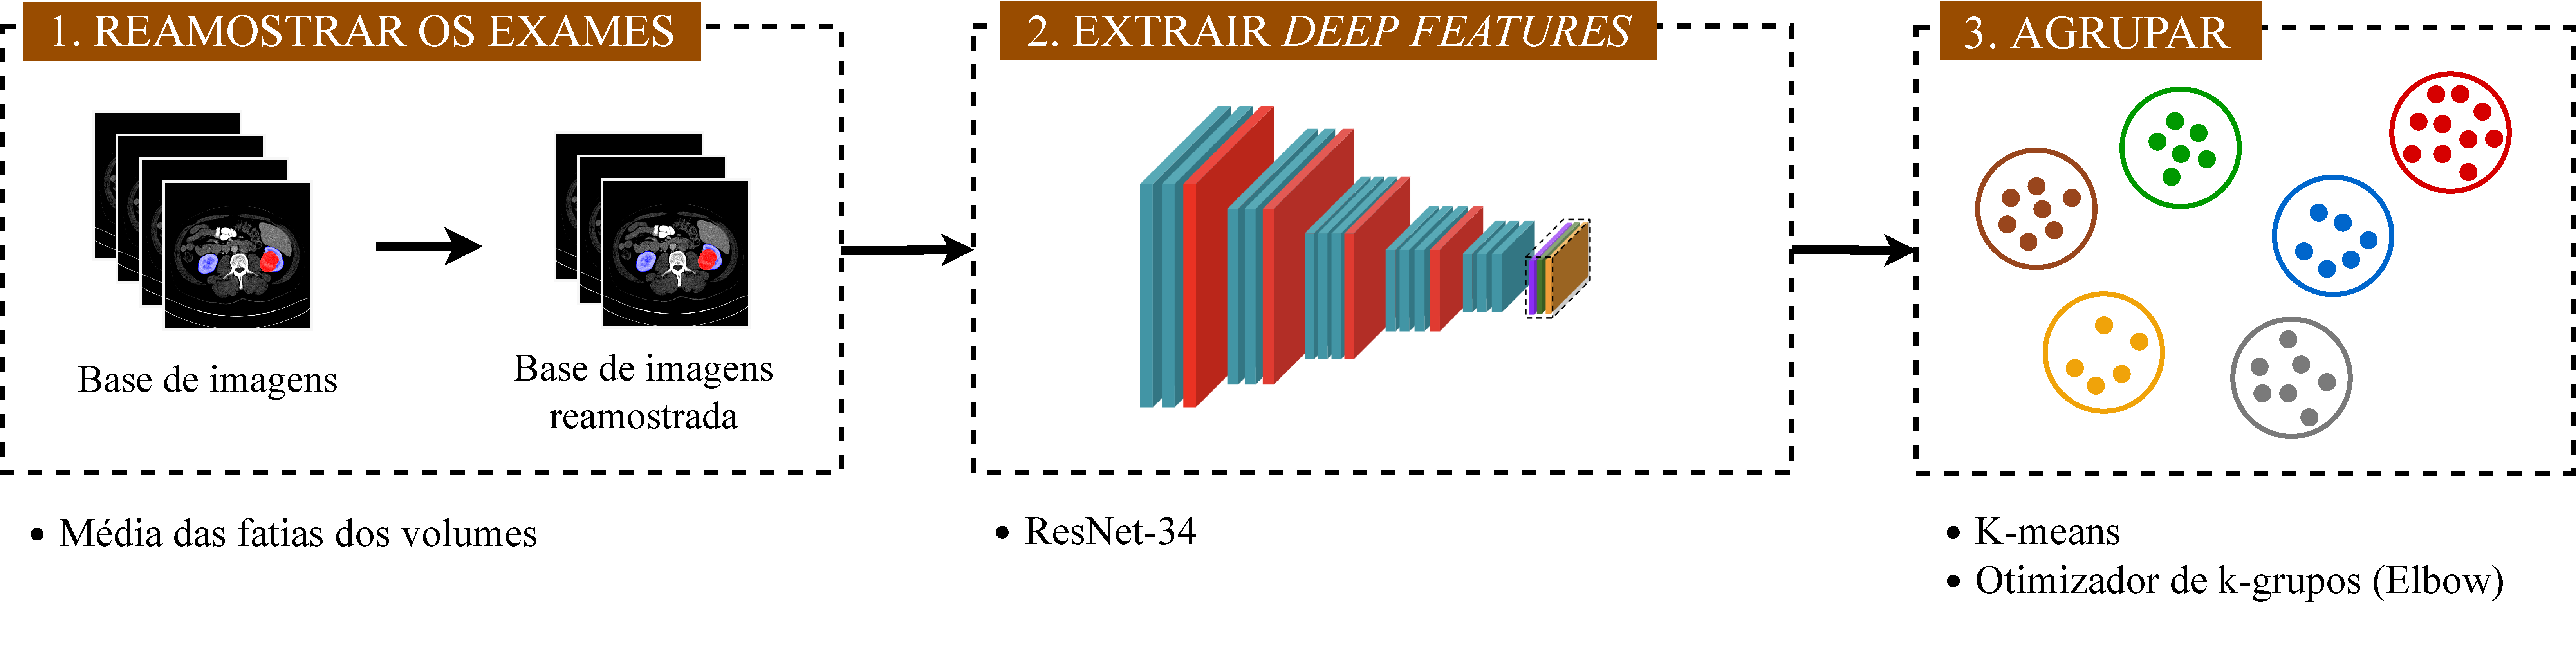
\includegraphics[width=1\textwidth]{figuras/distribuicao-proporcional-automatica.pdf}
    \label{fig:metodo-agrupar}
    \legend{Fonte: Elaborado pela autora.}
\end{figure}

Na primeira etapa, é realizada a técnica de reamostragem~\cite{dodgson1992image, 1372173} das tomografias, que é uma técnica matemática usada para criar uma nova versão da imagem com diferentes larguras, alturas e/ou profundidades em \textit{pixels}~\cite{dodgson1992image,sachs2001image}. Essa etapa é necessária porque os exames de TC podem ter diferentes quantidades de fatias e precisam ser reamostrados para o mesmo número de fatias para que os dados de entrada das etapas consecutivas sejam normalizados. Essa transformação dos dados é uma prática comum para evitar que o algoritmo fique enviesado para as variáveis com maior ordem de grandeza~\cite{kimble2015big}.

Para isso, padroniza-se o número de fatias em cada exame de TC por meio da operação de média, que consiste em calcular a quantidade total de fatias de tumores contidos na base de imagens (conjunto de treino e validação) e dividir pela quantidade de exames totais. Como resultado, obtém-se o valor médio de fatias. Posteriormente, a reamostragem é aplicada aos exames usando a informação do valor médio e interpolação linear, que produz uma superfície de intensidade garantida de forma contínua~\cite{andrews1976digital, dodgson1992image}. Por fim, com a técnica de reamostragem, todos os exames passam a ter um número n de fatias.

Na segunda etapa, são extraídas as \textit{deep features} que servirão como dados de entrada para a próxima etapa. As \textit{deep features} são extraídas pelos modelos ResNet-18, ResNet-34, ResNet-101~\cite{He7780459}, VGG-11, VGG-16~\cite{simonyan2014very}, DPN-131~\cite{chen2017dual} e Xception~\cite{chollet2017xception}. Esses modelos foram escolhidos por estarem consolidados na literatura para essa tarefa~\cite{8875911}, apresentando um alto desempenho, além de já terem sido pré-treinados. Todos os modelos realizam implicitamente a extração e seleção de características da região dos tumores. As características obtidas são extraídas da última camada de convolução de cada arquitetura. Os modelos são inicializados usando pesos pré-treinados aplicados à base de imagens ImageNet~\cite{deng2009imagenet}.

Finalmente, na terceira etapa, as características extraídas por cada modelo são utilizadas individualmente para realizar experimentos relacionados ao agrupamento de dados. O agrupamento é o processo de dividir os dados inteiros em grupos (também conhecidos como \textit{clusters}) com base nos padrões dos dados. Portanto, esta etapa visa agrupar os exames que possuam características semelhantes. Para isso, foi usado o K-means~\cite{macqueen1967some,hamerly2003learning}, que é o algoritmo de agrupamento mais comumente usado na literatura, para dividir o conjunto de dados em um conjunto de K-grupos. No K-means, cada grupo é representado pelo seu centro (isto é, centroide) que corresponde à média dos pontos atribuídos ao grupo. Em geral, as características extraídas de cada exame na segunda etapa são classificadas em grupos, de modo que tenham alta similaridade intraclasse e baixa similaridade interclasse.

Inicialmente, o modelo K-means é parametrizado em cada modelo de rede com diferentes números de K-grupos (de 2 a 20). Para cada valor de K, a inércia é calculada para medir o quão bem um conjunto de dados foi agrupado pelo K-means. A inércia é calculada medindo a distância entre cada ponto de dados e seu centroide, elevando essa distância ao quadrado e somando esses quadrados em um grupo. Posteriormente, o hiperparâmetro K é otimizado com o método do cotovelo (Elbow)~\cite{joshi2013modified}, que é frequentemente usado para encontrar o número ideal de grupos. Na Figura~\ref{fig:metodo-cotovelo} o valor da inércia para cada K associado é ilustrado usando o método do cotovelo. Pode-se observar que à medida que o número de grupos aumenta, o valor da inércia começa a diminuir. Além disso, o gráfico muda rapidamente em um ponto, criando uma forma de cotovelo, a partir do qual o gráfico começa a se mover quase paralelo ao eixo X. O método do cotovelo seleciona esse ponto do cotovelo no gráfico de inércia, pois o valor K correspondente é o valor K ótimo ou um número ótimo de grupos.

\begin{figure}[!ht]
    \centering
    \caption{Exemplo do método do cotovelo para seleção o número ideal de K-grupos.}
    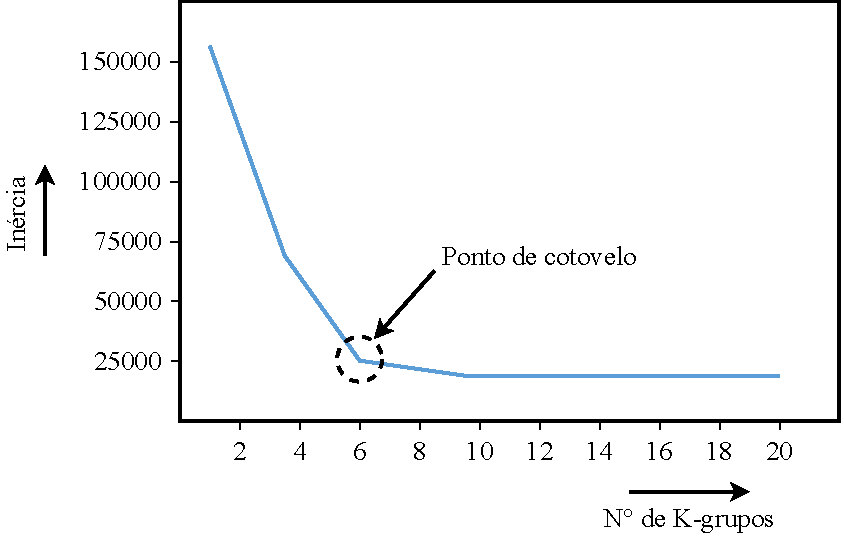
\includegraphics[width=0.75\textwidth]{figuras/metodo-cotovelo.pdf}
    \label{fig:metodo-cotovelo}
    \legend{Fonte: Elaborado pela autora.}
\end{figure}

Sabe-se que a ideia por trás de um bom agrupamento é ter um pequeno valor de inércia e um pequeno número de agrupamentos~\cite{joshi2013modified}. Portanto, este mesmo processo descrito acima é realizado para cada modelo de rede a fim de encontrar o seu melhor grupo. Posteriormente, dentre os modelos, deve-se selecionar aquele com menor valor de inércia, pois representará o modelo com melhor número de grupos. Isso completa o método para agrupar exames semelhantes.

Vale ressaltar que antes de aplicar as etapas descritas, o conjunto de teste é escolhido aleatoriamente da base de imagens. Em sequência, os exames de cada um dos grupos gerados pelo método proposto são selecionados aleatoriamente e distribuídos proporcionalmente entre os conjuntos de dados de treinamento e validação. Isso garante um modelo mais equilibrado, pois deve haver exames de todos os grupos de tumores em ambos os conjuntos de dados. Consequentemente, a generalização do modelo é aumentada.

Depois de distribuir proporcionalmente a base de imagens, alguns outros pré-processamentos foram aplicados para aprimorar as imagens de TC. Conforme já mencionado, esses outros pré-processamentos foram realizados em diferentes fluxos (descrito nas próximas subseções) para cada modelo de segmentação. Posteriormente, as imagens pré-processadas foram aplicadas para segmentar os rins e candidatos a tumores renais.

\subsection{Pré-processamentos Aplicados a Segmentação dos Rins}
\label{sec:pre-processamento-SR}

Antes de treinar o modelo de segmentação dos rins, os exames de TC são inicialmente submetidos a um processo de pré-processamento dividido em duas etapas. Essas etapas são ilustradas na Figura~\ref{fig:especificacao-janelamento}. A primeira etapa (Figura~\ref{fig:especificacao-janelamento} (a)) é a normalização das intensidades dos \textit{voxels} dos volumes de TC uma vez que as mesmas regiões dos rins podem ter intensidades muito diferentes em volumes diferentes, as quais podem dificultar uma eventual comparação das características de textura das regiões renais. Portanto, a especificação do histograma é aplicada para aproximar o histograma de um volume de TC ao histograma de um volume modelo escolhido aleatoriamente (fatia do volume modelo na Figura~\ref{fig:especificacao-janelamento}), de modo que ambos tenham uma distribuição dos \textit{voxels} semelhante~\cite{gonzalez2008digital}.

\begin{figure}[!ht]
    \centering
    \caption{Pré-processamento: (a) especificação do histograma; (b) janelamento.}
    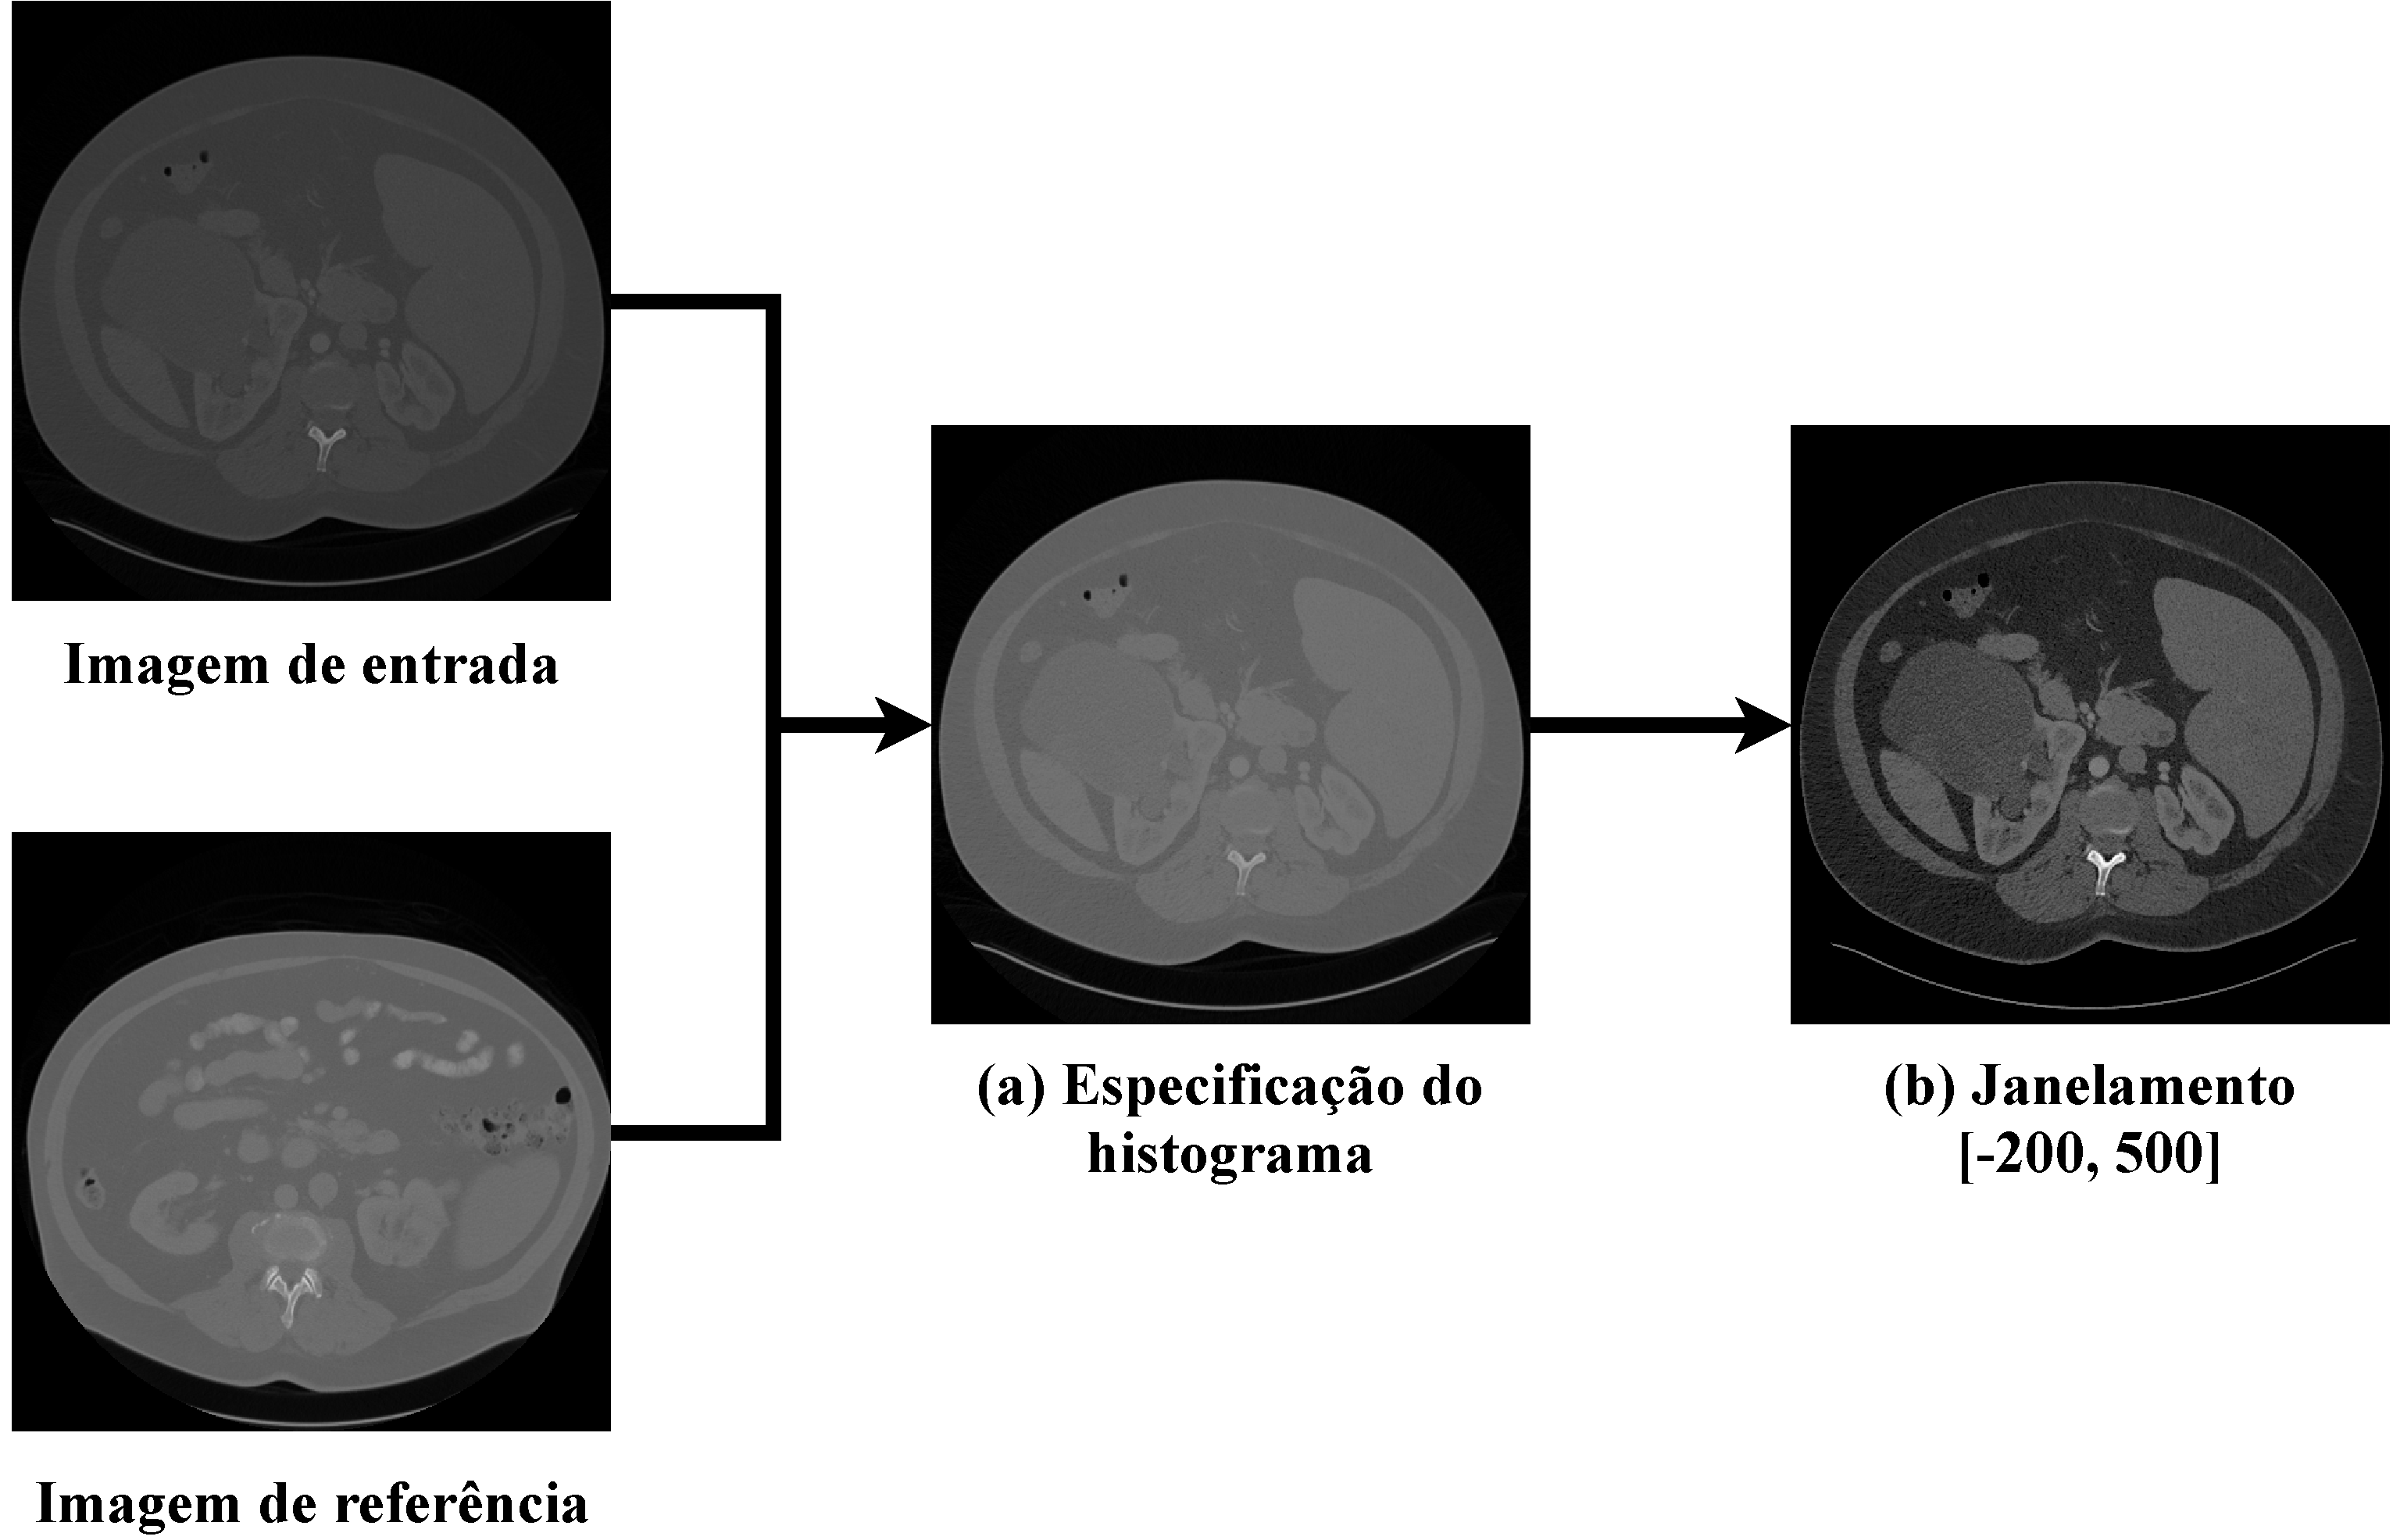
\includegraphics[width=0.85\textwidth]{figuras/especificacao-janelamento.pdf}
    \legend{Fonte: Elaborado pela autora.}
    \label{fig:especificacao-janelamento}
\end{figure}

Devido a existência de ossos, ar no intestino e outros órgãos, a faixa dos valores de TC nas imagens pode variar de -10.240 a mais de 18.000 HU. Valores tomográficos de tecidos moles, como rins e tumores renais, têm a mesma distribuição, variando de aproximadamente -200 HU a 500 HU \cite{Buzug2011, ADAMS2012277, yang2018automatic}. Portanto, na segunda etapa, os valores de intensidades dos volumes foram limitados para a faixa de [-200, 500] HU (Figura~\ref{fig:especificacao-janelamento} (b)). Este processo consiste em um janelamento, no qual se preserva os valores de \textit{voxels} que estão no intervalo entre -200 e 500 HU, e os \textit{voxels} com valores inferiores ou superiores a este intervalo são atribuídos os valores -200 e 500 HU, respectivamente. Isso melhora o contraste das imagens, facilitando a diferenciação das estruturas renais de outros órgãos~\cite{yang2018automatic,da2020kidney}. Em seguida, os valores de intensidade limitados foram normalizados entre 0 e 1. Esta transformação melhora a estabilidade da otimização, reduzindo a influência do problema de explosão de gradiente~\cite{Jason2019, Yash2021}.

\subsection{Pré-processamentos Aplicados à Segmentação Inicial de Candidatos a Tumores Renais}
\label{sec:pre-processamento-SRTR}

Para treinar os modelos de segmentação inicial a candidatos de tumores renais, as imagens de TC foram primeiramente submetidas ao pré-processamento de janelamento [-200, 500], que é o mesmo aplicado na segmentação de rins (Seção~\ref{sec:pre-processamento-SR}). A Figura~\ref{fig:janelamento} ilustra esse processo. Posteriormente, os valores de intensidade limitados com o janelamento também foram normalizados entre 0 e 1~\cite{Hands2017}.

\begin{figure}[!ht]
    \centering
    \caption{Pré-processamento: (a) imagem original; (b) janelamento.}
    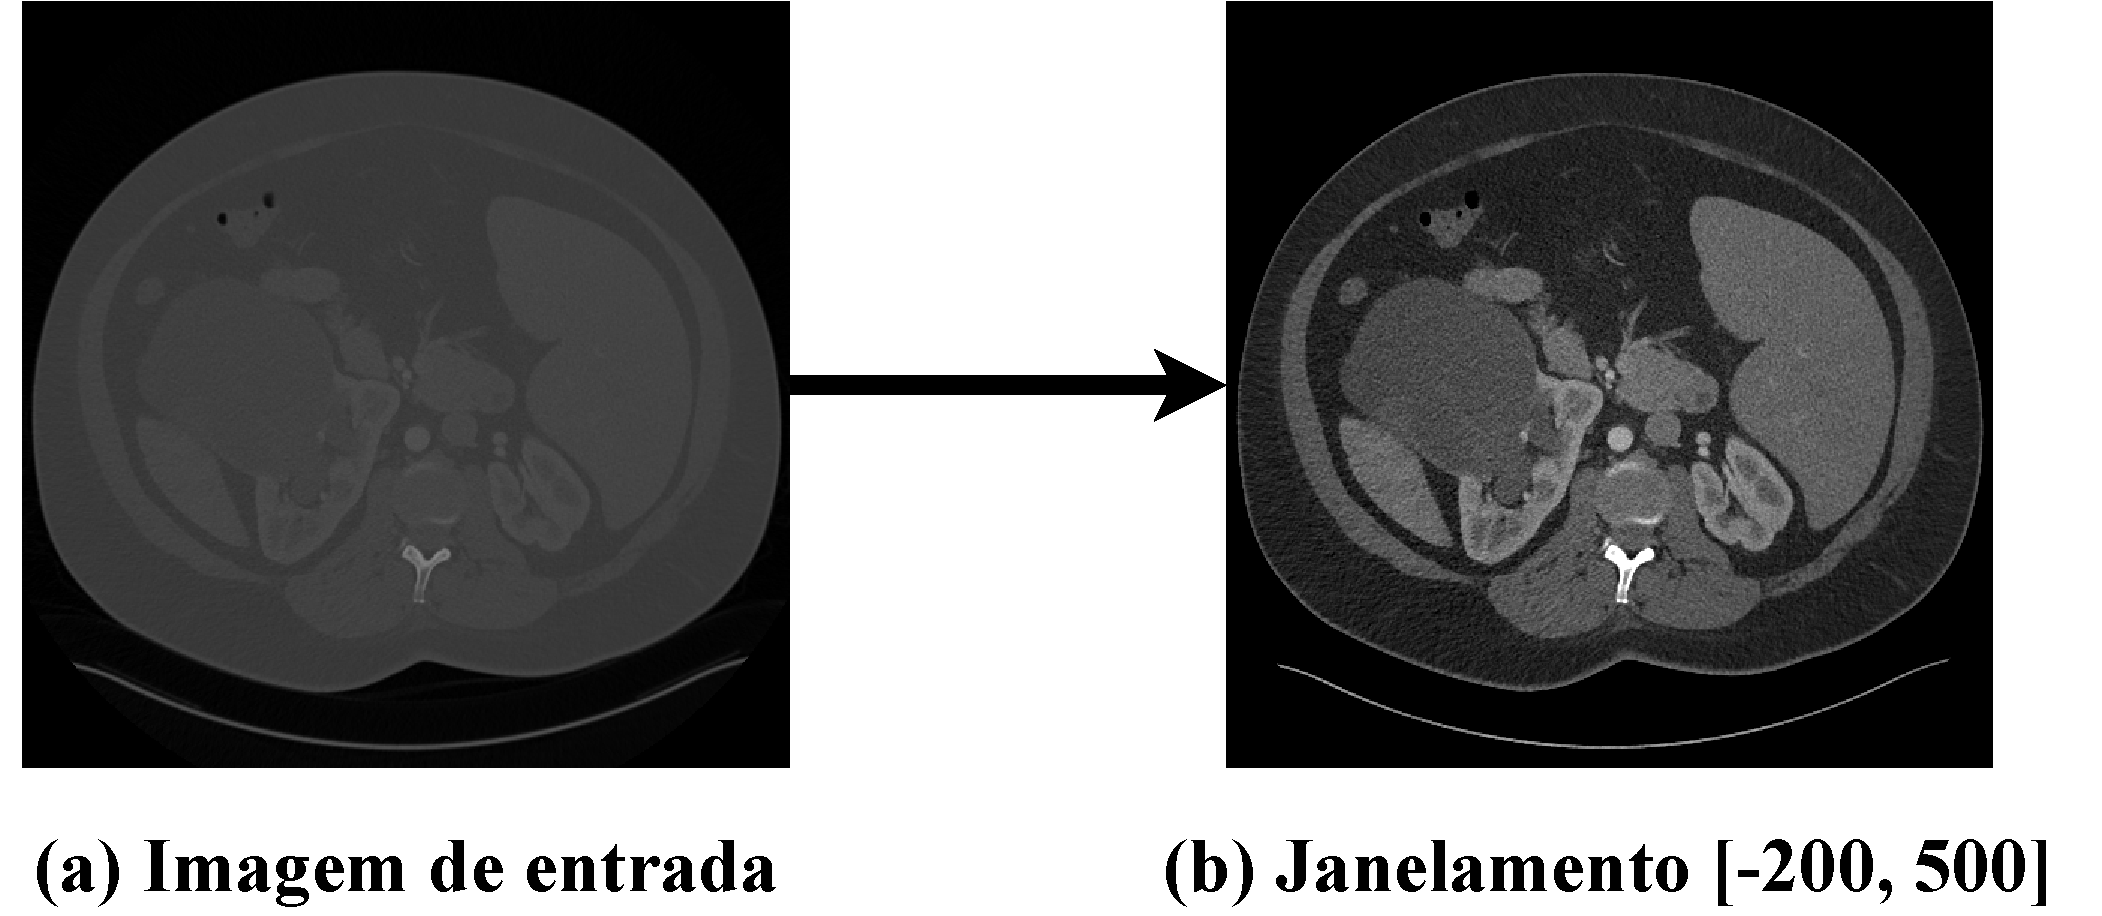
\includegraphics[width=0.75\textwidth]{figuras/janelamento.pdf}
    \legend{Fonte: Elaborado pela autora.}
    \label{fig:janelamento}
\end{figure}

\section{Segmentação Inicial}
\label{sec:metodo-segmentacao-inicial}

%Esta etapa visa a segmentação inicial dos rins e tumores renais após o pré-processamento das imagens de TC. Para isso, foram usados os modelos ResUNet e DeepLabv3+ para segmentar os rins e tumores renais, respectivamente. Após os modelos treinados, o processo de obter as segmentações dos rins e tumores renais ocorre em forma de cascata. Ou seja, os resultados da segmentação dos rins são usados como entrada para segmentar os tumores renais. Nas próximas subseções serão descritos os procedimentos para segmentar os rins e tumores renais.

Esta etapa visa a segmentação inicial dos rins e candidatos a tumores renais. Inicialmente, o modelo ResUNet foi usado para segmentar os rins. Para segmentar os candidatos a tumores renais, foram abordados dois estágios. O primeiro estágio usa o modelo DeepLabv3+ e o segundo estágio usa o modelo ResUNet. Nas próximas subseções serão descritos os procedimentos para segmentar os rins e candidatos a tumores renais.

\subsection{Segmentação dos rins usando a ResUNet}
\label{sec:metodo-segmentacao-dos-rins-ResUNet}

A ResUNet é uma arquitetura desenvolvida por \citeonline{ResUNet_8309343} para segmentação semântica. Foi inicialmente usada para extração de estradas a partir de imagens aéreas, mais tarde usada para várias outras aplicações, como segmentação de tumor cerebral e imagens humanas. Essa arquitetura é inspirada nos pontos fortes dos modelos de aprendizagem residual~\cite{He7780459} e U-Net~\cite{ronneberger2015u}. Em resumo, a rede é construída com unidades residuais e tem arquitetura semelhante à da U-Net. As vantagens deste modelo são duplas: em primeiro lugar, as unidades residuais facilitam o treinamento de redes profundas; em segundo, as ricas conexões de salto dentro da rede podem facilitar a propagação de informações renais, permitindo projetar redes com menos parâmetros e mais desempenho.

%Inicialmente, as fatias empilhadas em 3 canais são inseridas como uma imagem \textit{red-green-blue} (RGB).

A arquitetura ResUNet-101 usada neste trabalho é ilustrada na Figura~\ref{fig:arquitetura_ResUNet}. As imagens de entrada da rede são passadas por uma estrutura composta por três partes: codificação, ponte e decodificação. A primeira parte codifica a imagem de entrada em representações compactas. A última parte recupera as representações para uma segmentação semântica. A parte do meio serve como uma ponte conectando os caminhos de codificação e decodificação.

\begin{figure}[!ht]
    \centering
    \caption{Arquitetura ResUNet-101.}
    \includegraphics[width=1\textwidth]{figuras/arquitetura_ResUNet.png}
    \label{fig:arquitetura_ResUNet}
    \legend{Fonte: Elaborado pela autora.}
\end{figure}

A ResUNet usa unidades residuais como bloco de construção básico em vez de bloco convolucional simples. O caminho de codificação e decodificação é composto por quatro unidades residuais. As três partes são construídas com unidades residuais que consistem em dois blocos de convolução $3\times3$ e um mapeamento de identidade. Cada bloco de convolução inclui uma camada \textit{batch normalization}, uma camada de ativação ReLU e uma camada convolucional. O mapeamento de identidade conecta (adição) a entrada e a saída da unidade. No caminho de decodificação, antes de cada unidade, há uma deconvolução de mapas de características de nível inferior e uma concatenação com os mapas de características do caminho de codificação correspondente. Após o último nível do caminho de decodificação, uma convolução $1\times1$ e uma camada de ativação sigmoide são usadas para projetar os mapas de características para a segmentação dos rins.

Resumidamente, a abordagem residual consiste em propagar informações sobre camadas, inserindo conexões de atalho entre as camadas de entrada e saída. Essas conexões de atalho simplesmente executam o mapeamento de identidade e suas saídas são adicionadas às saídas das camadas empilhadas. Assim, a inserção dos mapas de entrada na saída de cada camada evita que o conjunto de operações de \textit{pooling} reduza as informações necessárias contidas nas imagens da base. Portanto, este modelo foi escolhido devido ao seu alto desempenho para segmentação renal, uma vez que as informações são propagadas com a abordagem residual, retendo e agregando características renais relevantes.

%Os blocos residuais criam um mapeamento de identidade para ativações anteriores na rede para impedir o problema de degradação de desempenho associado a arquiteturas neurais profundas.
%No entanto, ResNets profundos são capazes de formar uma função de identidade que mapeia para uma ativação anterior na rede quando a ativação de uma camada específica tende a zerar mais profundamente na rede.
%A melhoria do desempenho é alcançada sempre que as camadas extras aprendem algumas informações significativas dos dados. Enquanto, a presença de blocos residuais evita a perda de desempenho sempre que as ativações tendem a desaparecer ou explodir.

%quando combinado com DeepLabv3 + 2.5D, permitiu a exploração de novos recursos, que possibilitaram o aprendizado de representações tumorais a partir da captura de suas informações contextuais, como diferentes formas e tamanhos.

\subsubsection{Treinamento da ResUNet 2.5D}
\label{sec:treinamento-ResUNet}

A rede é treinada com imagens de TC no tamanho original de $512\times512$ \textit{pixels}. O modelo usa uma abordagens 2.5D, que consiste em passar como entrada da rede uma pilha de três fatias consecutivas (anterior, central e posterior) e a máscara referente à fatia central com as marcações dos rins. Para analisar todo o volume de TC, o mesmo processo descrito foi realizado deslizando uma janela de tamanho $3\times3$ com um passo igual a 1 sobre as fatias. A saída da ResUNet é a máscara para a segmentação da fatia central da pilha. Um exemplo de fatias de entrada da rede usando a abordagem 2.5D é mostrado na Figura~\ref{fig:abordagem-2.5D}.

%Posteriormente, as segmentações de cada fatia são combinadas para construir o volume 3D do resultado de cada caso no conjunto de dados da tese.

\begin{figure}[!ht]
    \centering
    \caption{Abordagem 2.5D: exemplo de imagens de entrada.}
    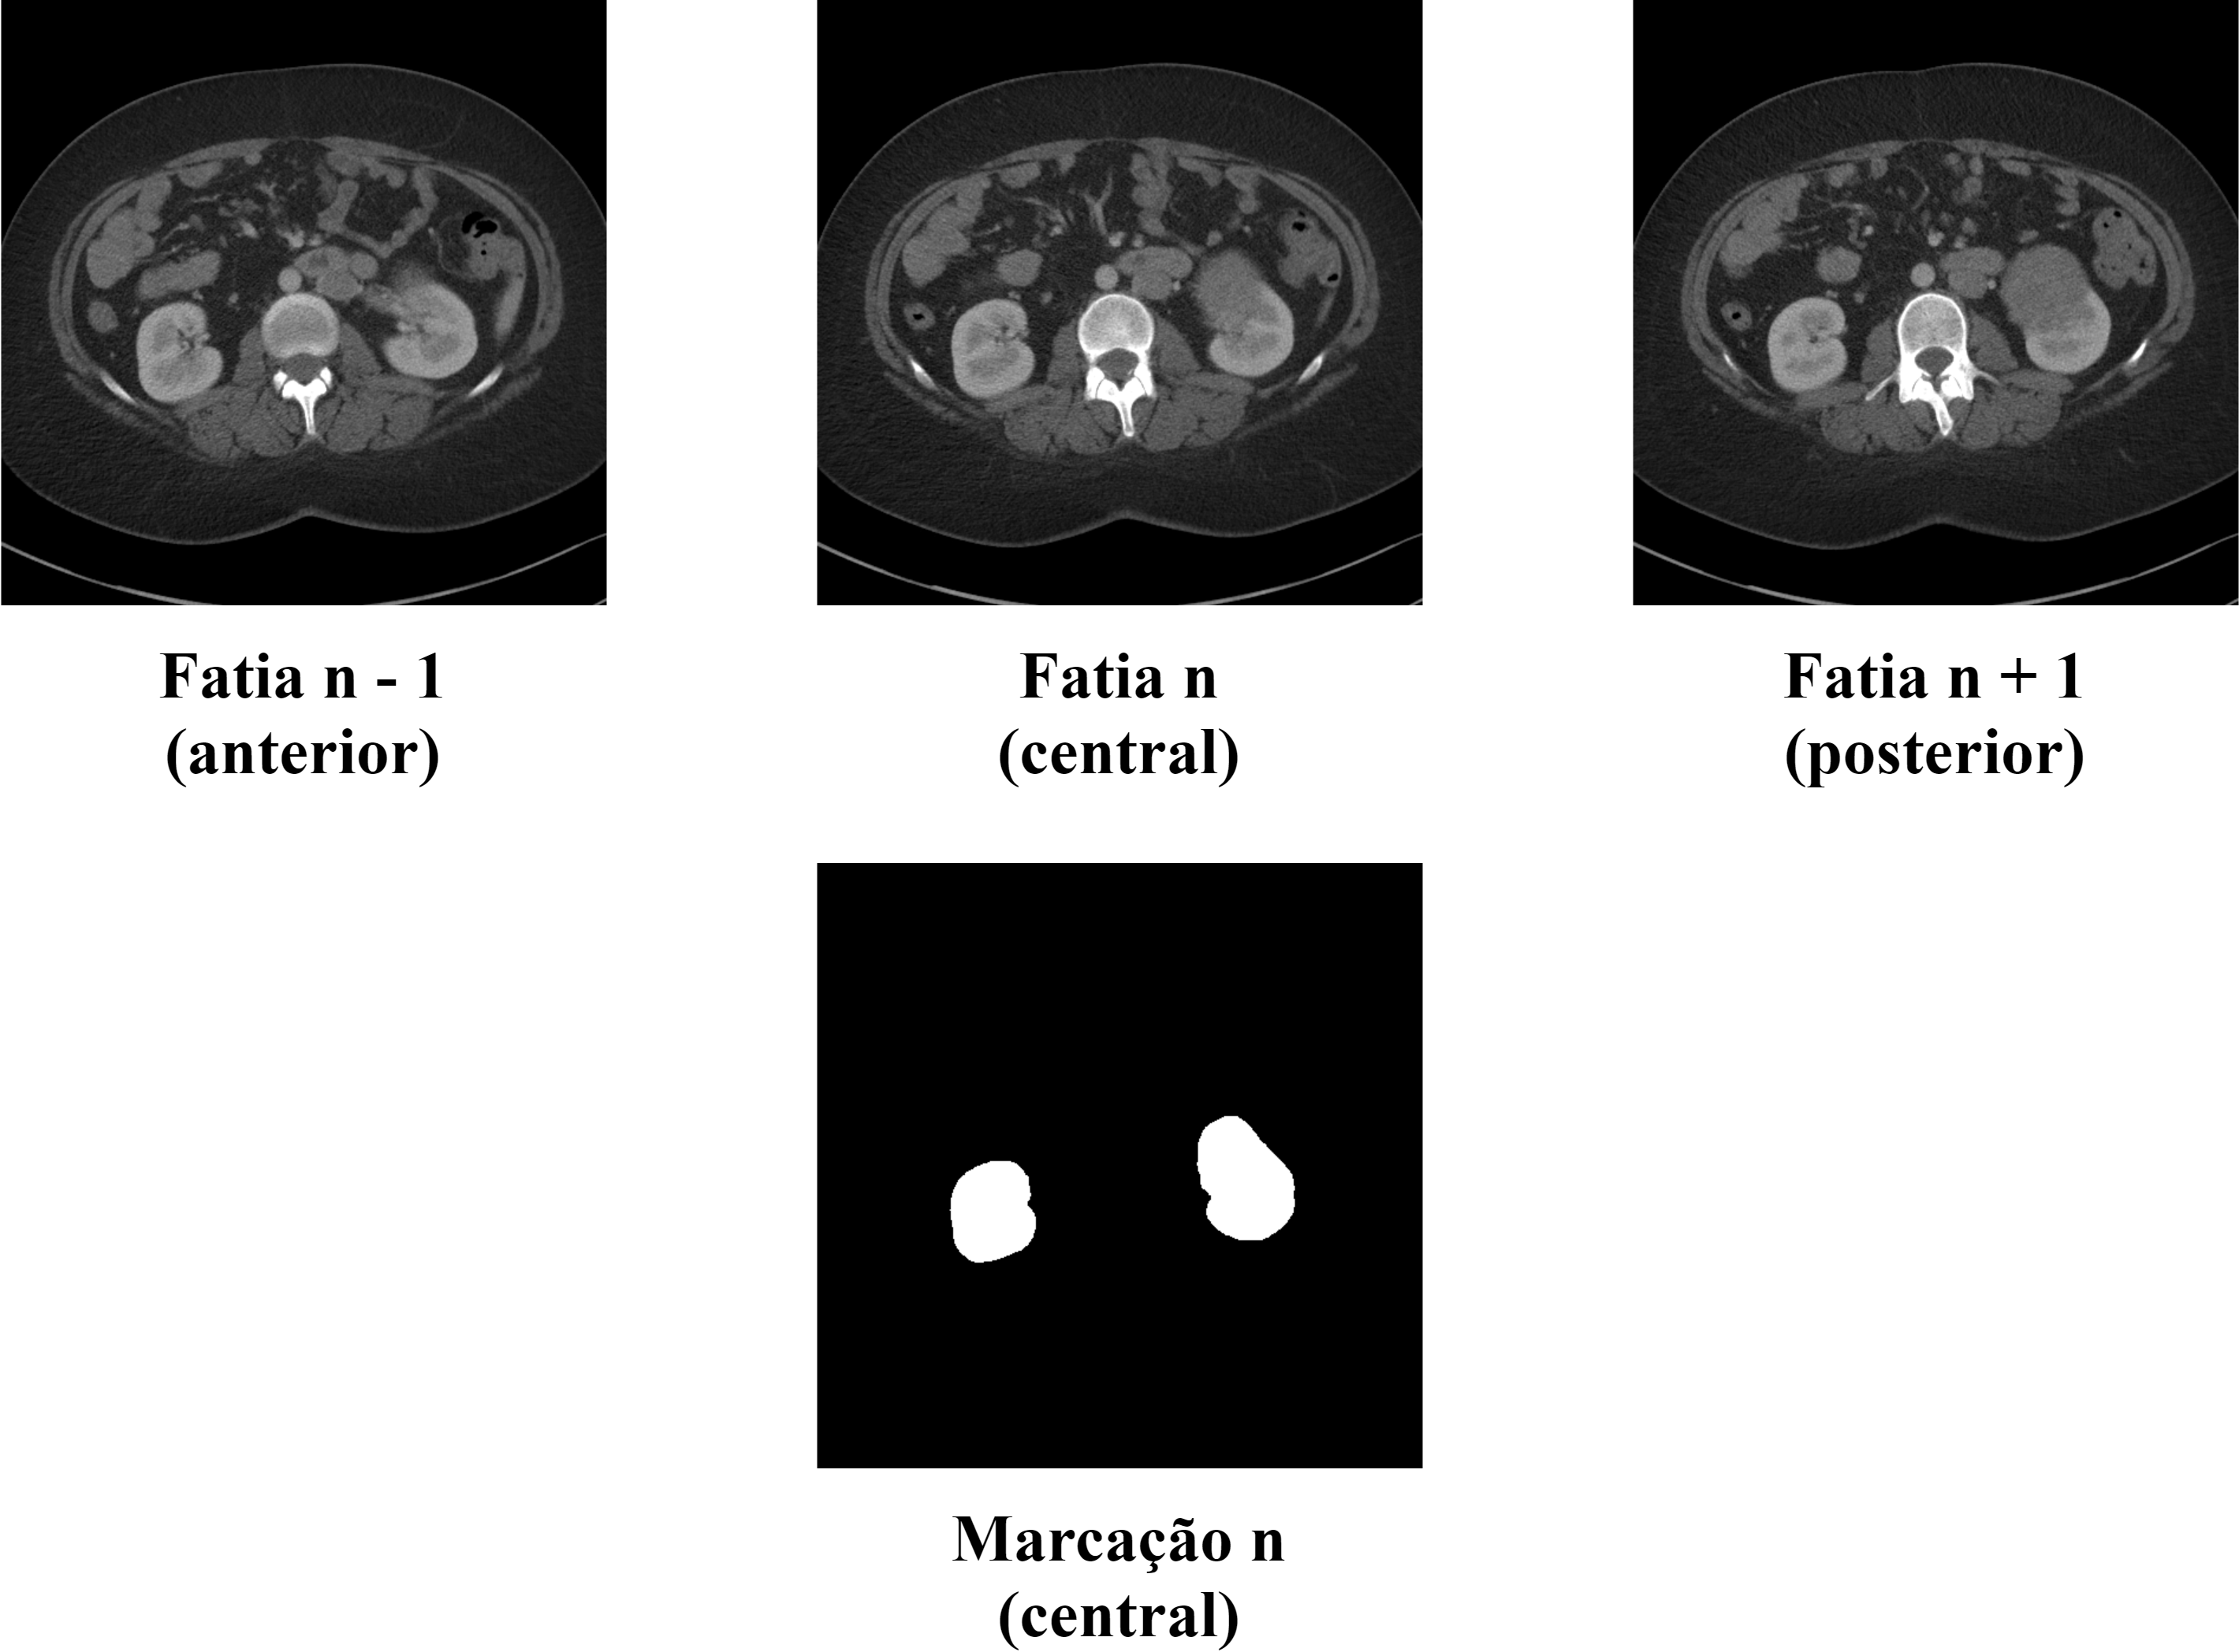
\includegraphics[width=0.8\textwidth]{figuras/abordagem-2.5D-entrada.png}
    \label{fig:abordagem-2.5D}
    \legend{Fonte: Elaborado pela autora.}
\end{figure}

Uma das vantagens da abordagem 2.5D é que pode-se usar informações espaciais das fatias vizinhas para identificar o objeto de interesse, aumentando as chances de segmentação bem-sucedida e reduzindo os falsos positivos. Isso só foi possível devido à natureza da abordagem 2.5D, que possui conexões entre as fatias do volume de TC. 

Além da abordagem 2.5D, um balanceamento de fatias de rins e não rins foi usado nos conjuntos de treinamento e validação. O balanceamento consistiu em usar as fatias com rins e adicionar a mesma quantidade de fatias sem rins e depois retirar o excesso de fatias sem rins. Essa estratégia ajuda o modelo de aprendizado profundo a detectar se uma fatia tem rins ou não, a qual reduziu consideravelmente os falsos positivos.

%o que foi equivalente a 28.732 imagens (14.366 com rins e 14.366 sem rins) e as fatias em excesso sem rins foram removidas (11.186 fatias)

Por fim, o treinamento da ResUNet 2.5D foi inicializado usando os pesos pré-treinados aplicados à base de imagens ImageNet~\cite{deng2009imagenet}. Essa prática ajuda a minimizar o tempo de treinamento e economizar recursos de \textit{hardware}.

\subsection{Segmentação Inicial de Candidatos a Tumores Renais}
\label{sec:metodo-segmentacao-inicial-candidatos-tumores-renais}

Esta etapa visa a segmentação inicial de candidatos a tumores renais. Para isso, foi dividida em dois estágios: o primeiro estágio usa os resultados da segmentação inicial dos rins como entrada para segmentar os candidatos a tumores renais usando o modelo DeepLabv3+; o segundo estágio usa outro modelo ResUNet para segmentar candidatos a tumores renais dentro da região abdominal (imagem completa). Mais detalhes de cada estágio são descritos nas próximas subseções.

\subsubsection{Candidatos de Tumores Renais na Região Renal}
\label{sec:metodo-candidatos-tumores-renais-regiao-renal}

Como já mencionado, este primeiro estágio visa obter candidatos a tumores renais dentro da região renal. Para isso, os resultados adquiridos na etapa de segmentação de rins foram usados como entrada para segmentar os candidatos a tumores renais. Neste estágio, o modelo de aprendizado profundo DeepLabv3+ (Seção~\ref{sec:deeplabv3+}) foi adaptado para realizar a segmentação das regiões tumorais. Esta adaptação consiste em remover o codificador padrão (Xception~\cite{chollet2017xception}) da DeepLabv3+, pela arquitetura de rede de caminho duplo (\textit{Dual Path Network} - DPN)-131. Para isso, foi necessário remover a camada totalmente conectada da DPN-131 para funcionar como um extrator de características no modelo proposto.

A DPN é uma rede de classificação que apresenta uma topologia de caminhos de conexão interna. A DPN compartilha as vantagens da Rede Residual (\textit{Residual Network} - ResNet)~\cite{He7780459}, que permite a reutilização de recursos, e da Rede Densamente Convolucional (\textit{Densely Convolutional Network} - DenseNet)~\cite{Huang8099726}, que explora os novos recursos que são importantes para o aprendizado de boas representações~\cite{chen2017dual}. A DPN-131 empilha vários blocos \textit{dual path} modularizados, conforme mostrado na Figura~\ref{fig:arquitetura_DPN}. Inicialmente, uma convolução 7 × 7 é aplicada, seguida de \textit{batch normalization}, função de ativação ReLU e \textit{max-pooling} $3\times3$. A estrutura de cada bloco é projetada com um estilo de gargalo~\cite{He7780459}, que começa com uma camada convolucional $1\times1$, seguida por uma $3\times3$ e finalizando com uma $1\times1$.

Assim, a saída da última camada convolucional $1\times1$ é dividida em duas partes. Na primeira parte, é adicionado ao caminho residual e, na segunda parte, é concatenado com o caminho densamente conectado. Em outras palavras, as redes residuais adicionam os recursos de entrada aos recursos de saída por meio do caminho residual, e as redes densas usam um caminho densamente conectado para concatenar recursos de entrada com recursos de saída, permitindo que cada bloco receba informações de todos os blocos anteriores. A camada de convolução agrupada na segunda camada é usada como ResNeXt~\cite{xie2017aggregated}, aumentando a capacidade de aprendizado de cada bloco.

\begin{figure}[!ht]
    \centering
    \caption{Arquitetura DPN-131.}
    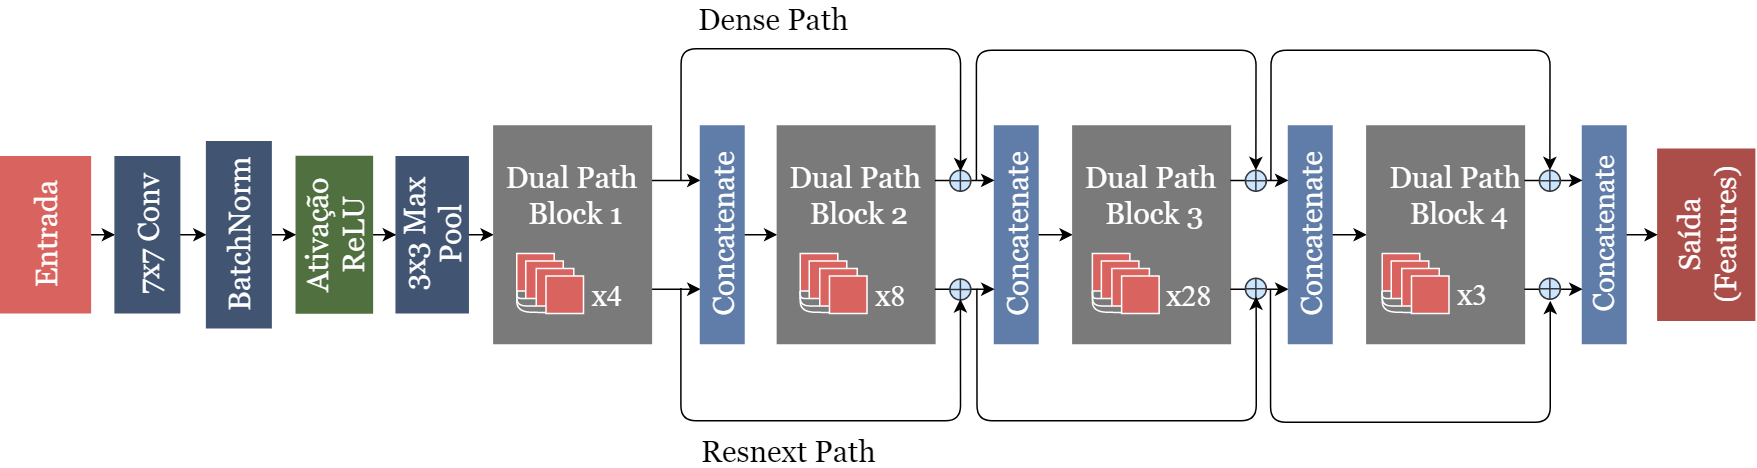
\includegraphics[width=1\textwidth]{figuras/arquitetura_DPN.png}
    \legend{Fonte: Elaborado pela autora.}
    \label{fig:arquitetura_DPN}
\end{figure}

Como a arquitetura DPN-131 padrão foi usada como o codificador da DeepLabv3+, foi necessário remover a camada totalmente conectada do DPN-131 para funcionar como um extrator de características, conforme visto na Figura~\ref{fig:arquitetura_DPN}. Além disso, embora várias funções de ativação tenham sido aplicadas com redes profundas para obter alto desempenho~\cite{8936083, GOCERI2021104118}, foi usada a função ReLU devido à sua eficiência na segmentação da base de imagens e baixo custo computacional.

Finalmente, pode ser observado na Figura~\ref{fig:arquitetura_DeepLabv3+DPN} a arquitetura DeepLabv3+ usada para a segmentação a candidatos de tumores renais. A escolha da DPN-131 foi feita por ser eficiente, introduzindo uma nova topologia de caminhos de conexão internamente. Além disso, vale ressaltar que a DeepLabv3+ é um modelo de aprendizado profundo de última geração capaz de refinar os resultados da segmentação com foco especial nos limites do objeto. Outro ponto importante é que a rede extrai mapas de características densos para capturar contextos de longo alcance (informações contextuais de pixels mais distantes), melhorando a tarefa de segmentar os diferentes tamanhos e formas dos tumores encontrados na base de imagens. Portanto, a combinação resultou em um codificador-decodificador robusto, com alto desempenho para segmentação a candidatos de tumores renais.

\begin{figure}[!ht]
    \centering
    \caption{Arquitetura DeepLabv3+.}
    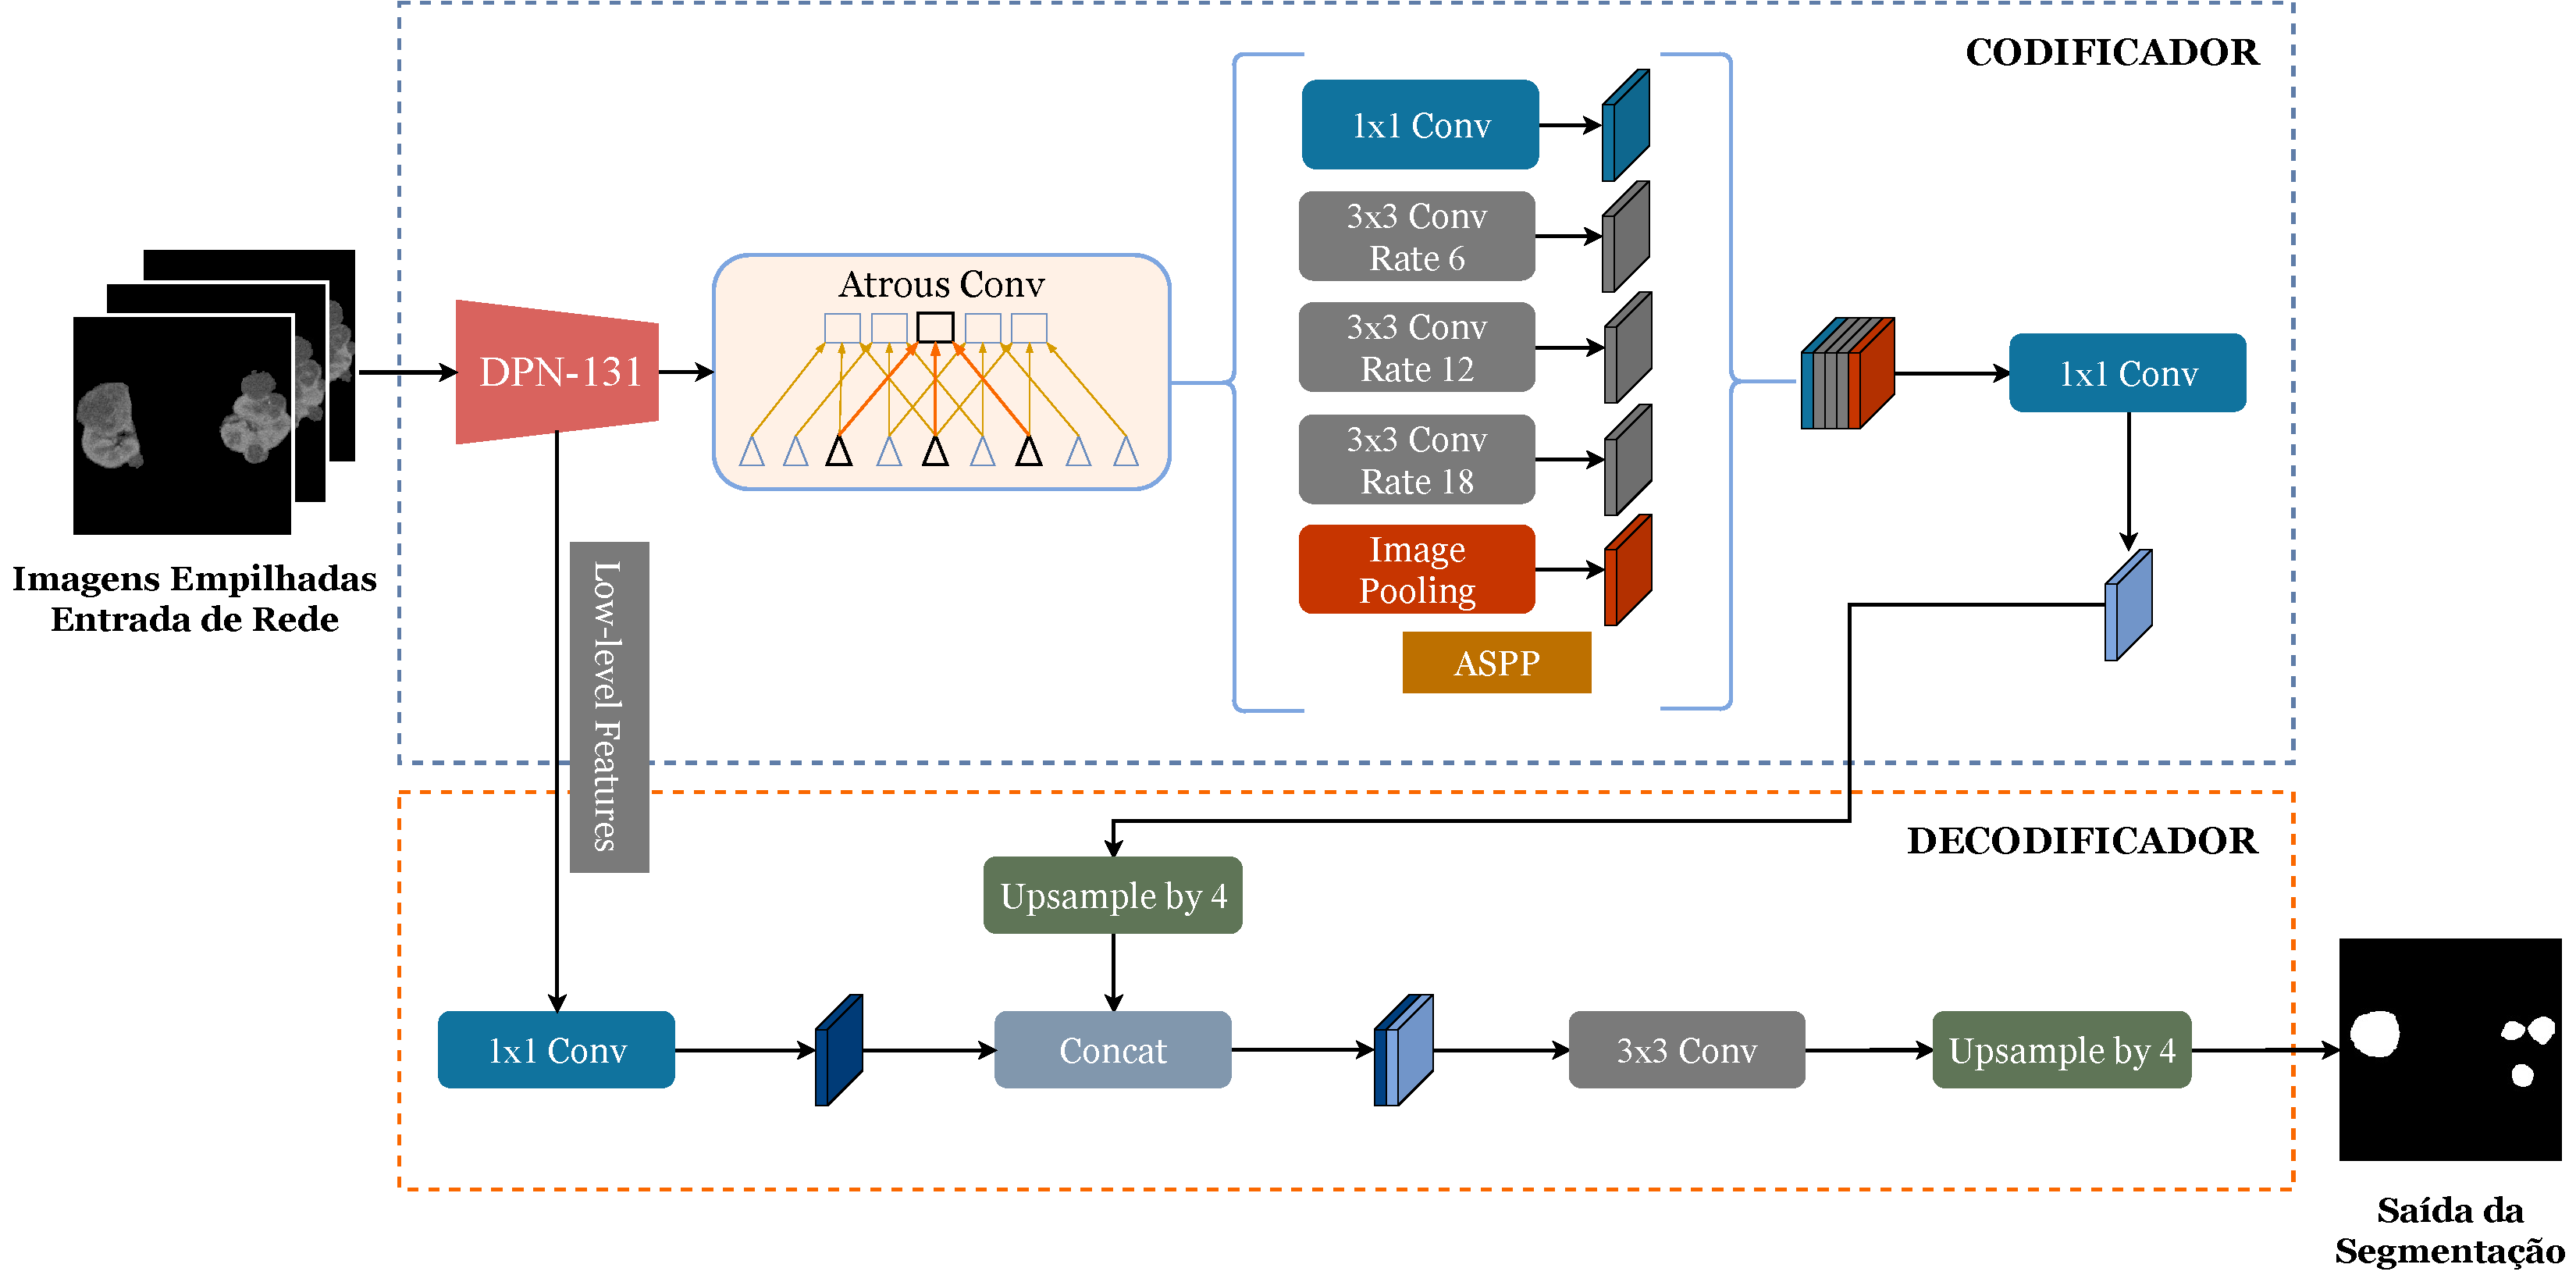
\includegraphics[width=1\textwidth]{figuras/arquitetura_Deeplabv3+DPN.pdf}
    \label{fig:arquitetura_DeepLabv3+DPN}
    \legend{Fonte: Adaptado de~\cite{chen2018encoder}.}
\end{figure}

\subsubsubsection{Treinamento da DeepLabv3+ 2.5D}
\label{sec:treinamento-DeepLabv3+}

Antes de realizar o treinamento, as regiões renais foram inicialmente recortadas automaticamente nas imagens de TC. Os rins foram encontrados usando a marcação do especialista e aplicando uma caixa delimitadora 3D que envolvesse os dois rins (Figura~\ref{fig:recorte} (a)). Então, o volume é cortado para o valor correspondente à caixa delimitadora 3D (Figura~\ref{fig:recorte} (b)). Posteriormente, um redimensionamento proporcional para $256\times256$ \textit{pixels} foi aplicado às imagens cortadas maiores que 256 \textit{pixels} de altura ou largura (Figura~\ref{fig:recorte} (c)). Finalmente, as imagens foram centralizadas com um tamanho final de $256\times256$ \textit{pixels} e apenas a textura da região do rim é mantida (Figura~\ref{fig:recorte} (d)) para a segmentação da região dos tumores. Todo esse processo foi realizado porque havia muitas regiões irrelevantes (outros órgãos) para capturar características. Também foi necessário devido às limitações de \textit{hardware}, já que a arquitetura é profunda e requer memória considerável para representar todos os mapas de características.

\begin{figure}[!ht]
    \centering
    \caption{Delimitação da região de interesse.}
    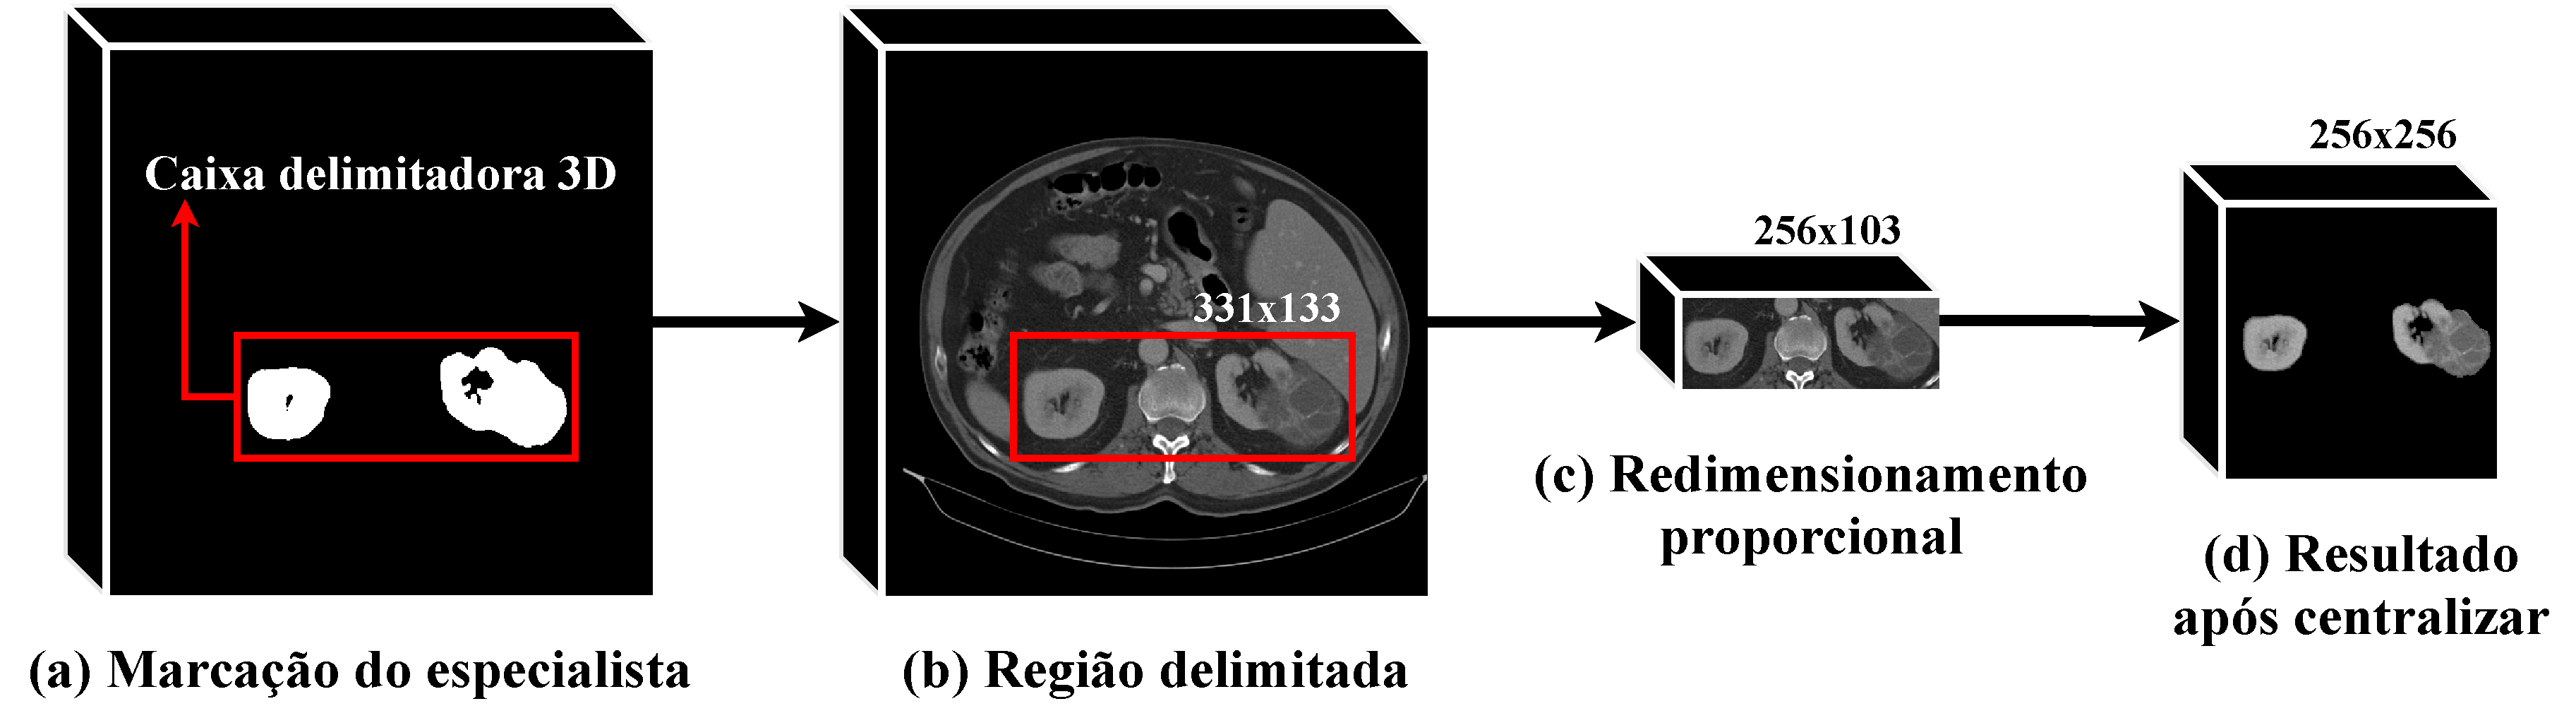
\includegraphics[width=1\textwidth]{figuras/recorte.pdf}
    \legend{Fonte: Elaborado pela autora.}
    \label{fig:recorte}
\end{figure}

Finalmente, o modelo DeepLabv3+ foi treinado usando abordagem 2.5D, conforme descrito na Seção~\ref{sec:treinamento-ResUNet}. No entanto, foram passadas para entrada da rede três fatias consecutivas da região dos tumores e a máscara referente a fatia central com as marcações dos tumores.

Nos experimentos realizados também aplicou-se o balanceamento de fatias (Seção~\ref{sec:treinamento-ResUNet}) nos conjuntos de treinamento e validação. Entretanto, o balanceamento de fatias para o modelo de segmentação a candidatos de tumores renais na região renal consistiu em usar as fatias com tumores e somar a mesma quantidade de fatias sem tumores e, posteriormente, remover as fatias excedentes sem tumores. Isso reduziu bastante os falsos positivos, devido às regiões que são muito semelhantes a tumores renais, como cistos.

%totalizando 9.814 imagens (4.907 com tumores renais e 4.907 sem tumores renais), e as fatias excedentes sem tumores renais foram removidas (4.552 fatias)

A inicialização do treinamento da DeepLabv3+ 2.5D também utilizou os pesos pré-treinados aplicados à base de imagens ImageNet~\cite{deng2009imagenet}.

%A entrada da rede, são fatias de TC empilhadas em 3 canais (RGB). Em seguida, as imagens passam por uma estrutura de codificador-decodificador.

\subsubsection{Candidatos de Tumores Renais na Região Abdominal}
\label{sec:metodo-candidatos-tumores-renais-regiao-abdominal}

O segundo estágio também visa segmentar candidatos a tumores renais. No entanto, toda a região abdominal é analisada. Isso é feito porque no primeiro estágio o modelo está limitado a segmentar candidatos a tumores renais apenas dentro da região renal resultante da segmentação inicial dos rins. Esse procedimento pode acabar não trazendo os resultados desejados por falta de informações contextuais e porque algumas regiões renais não foram obtidas na segmentação inicial dos rins. Logo, essas regiões poderiam ter tumores renais e acabaram não tendo a possibilidade de segmentá-los.

Portanto, o segundo estágio tem o objetivo de segmentar os candidatos a tumores renais na região abdominal, analisando mais informações contextuais em uma região mais ampla. Vale ressaltar que essa técnica é mais suscetível a falsos positivos, pois o tumor renal não tem um formato padronizado, o que pode causar confusão com outras estruturas (órgãos). Entretanto, o modelo traz resultados interessantes, pois é capaz de segmentar tumores renais que não haviam sido segmentados no estágio anterior.

Dessa forma, um segundo modelo de aprendizado profundo é treinado para realizar a segmentação de candidatos a tumores renais na região abdominal. Para isso, é usado o modelo ResUNet que é a mesma arquitetura descrita na Seção~\ref{sec:metodo-segmentacao-dos-rins-ResUNet}. No entanto, o treinamento do modelo é realizado usando apenas as marcações dos tumores renais, mas com informações mais ampla (regiões abdominais). Ou seja, o modelo é especializado nas segmentações dos tumores nas imagens de TC. Além disso, o modelo também usa a abordagem 2.5D e balanceamento de fatias (Seção~\ref{sec:treinamento-DeepLabv3+}). 

A Figura~\ref{fig:candidatos-de-tumores-renais} ilustra a segmentação inicial dos candidatos a tumores renais em uma imagem de TC aplicada à entrada dos modelos (DeepLabv3+ e ResUNet). Na Figura~\ref{fig:candidatos-de-tumores-renais}~(a) apresenta a marcação do especialista. O resultado da etapa de candidatos a tumores renais na região renal é mostrado na Figura~\ref{fig:candidatos-de-tumores-renais} (b). Finalmente, os candidatos a tumores renais na região abdominal que podem não ter sido segmentados no primeiro estágio são ilustrados na Figura~\ref{fig:candidatos-de-tumores-renais} (c). No entanto, nota-se que alguns fragmentos semelhantes a tumores renais também foram segmentados.

\begin{figure}[!ht]
    \centering
    \caption{Candidatos a tumores renais: (a) marcação do especialista; (b) candidatos de tumores renais na região renal; (c) candidatos de tumores renais na região abdominal.}
    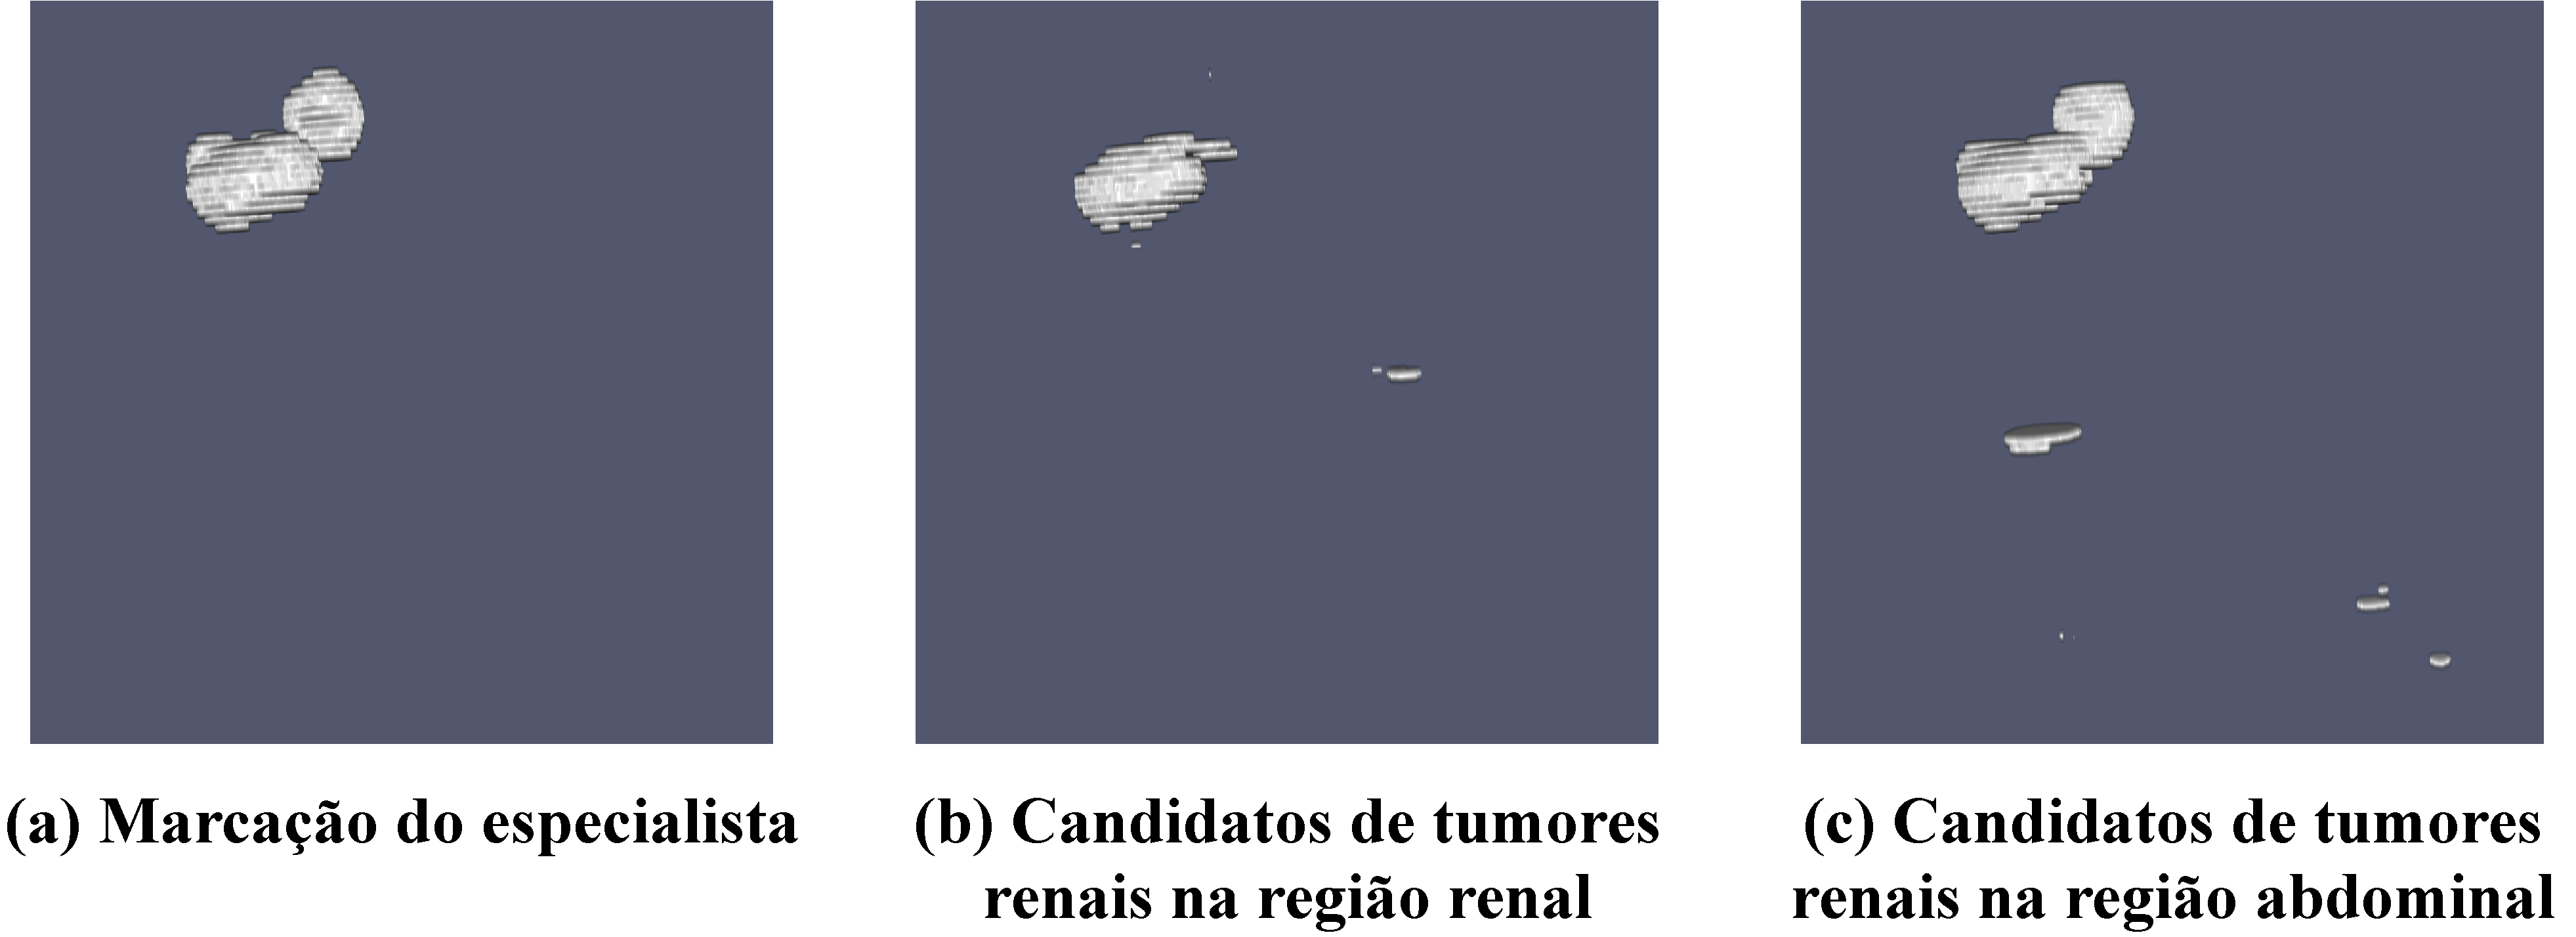
\includegraphics[width=0.9\textwidth]{figuras/candidatos-de-tumores-renais.pdf}
    \legend{Fonte: Elaborado pela autora.}
    \label{fig:candidatos-de-tumores-renais}
\end{figure}

\section{Reconstrução dos Tumores Renais}
\label{sec:metodo-reconstrucao-dos-tumores-renais}

%Em bons cenários, em que os pacientes têm tumores renais bem definidos, apenas a segmentação dos tumores é suficiente para alcançar bons resultados. Porém, em casos difíceis como surgimento de cistos, texturas homogêneas e tumores em estágios avançados (Figura~\ref{fig:casos-dificeis}), o modelo acaba não segmentando bem os tumores renais. Isso se deve ao fato de que o modelo usa informações de textura para realizar a segmentação e, portanto, a diferença de contraste em uma mesma região dos tumores é um fator importante. A Figura xxx ilustra um caso em que a segmentação inicial é comprometida pela situação acima mencionada.

Em bons cenários, onde a segmentação inicial dos rins foi capaz de obter grande parte da região renal, e em que os pacientes apresentam tumores bem definidos, apenas o primeiro estágio é suficiente para alcançar bons resultados. Porém, em casos difíceis como surgimento de cistos, texturas homogêneas, tumores em estágios avançados (Figura~\ref{fig:casos-dificeis}) e perda de regiões renais na segmentação inicial dos rins, o modelo acaba não segmentando bem os tumores.

\begin{figure}[!ht]
    \centering
    \caption{Exemplos de casos difíceis. Rins marcados em azul e tumores renais em vermelho.}
    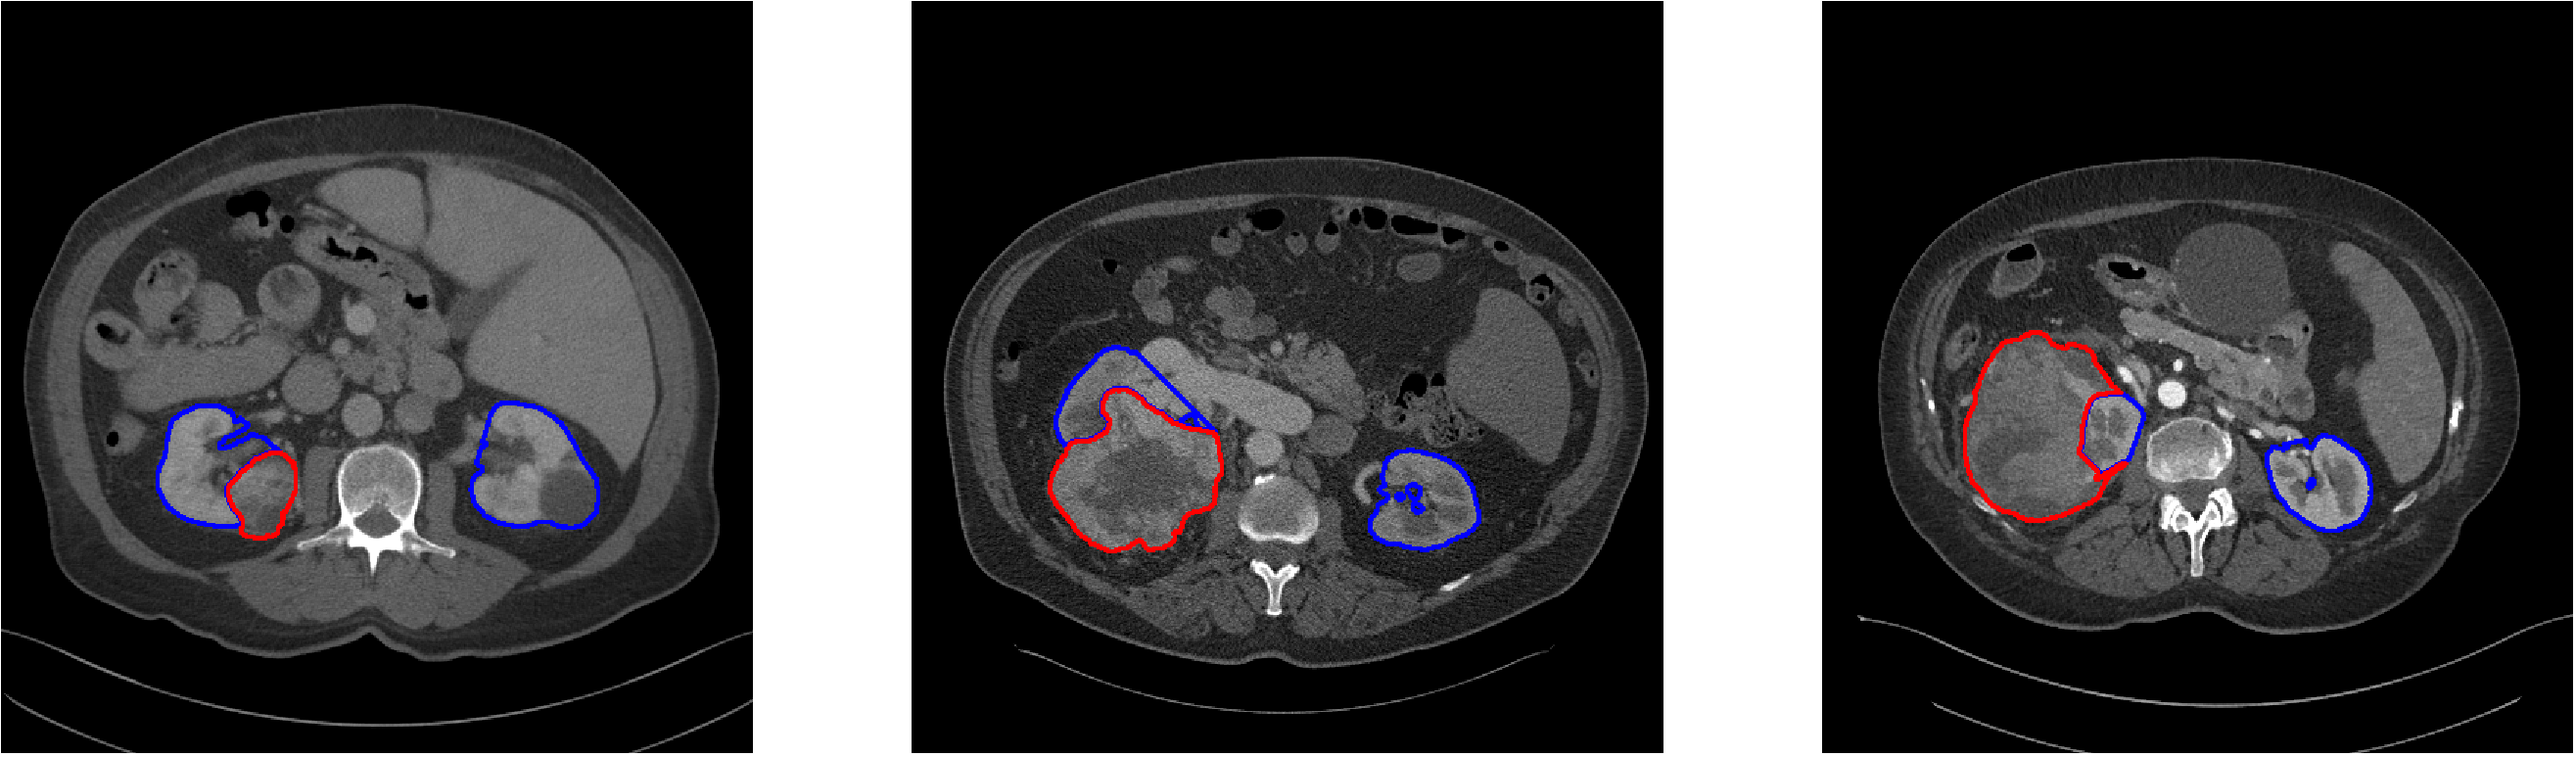
\includegraphics[width=1\textwidth]{figuras/casos-dificeis.pdf}
    \legend{Fonte: Elaborado pela autora.}
    \label{fig:casos-dificeis}
\end{figure}

%A fim de solucionar esses casos particulares e, portanto, desenvolver um modelo de segmentação mais robusto, um segundo modelo de aprendizado profundo é treinado para realizar uma reconstrução dos tumores renais. Esta etapa é dividida em duas subetapas: segmentação dos tumores renais na região de interesse, com ResUNet; e a união da primeira subetapa supracitada com o resultado da segmentação inicial dos tumores renais.

%Com as segmentações adquiridas, o resultado da etapa de reconstrução é obtida pela união da segmentação inicial dos tumores renais e reconstrução dos tumores renais. Para isso, foi realizada uma operação binária (OU) nas duas máscaras de segmentação. A Figura~\ref{fig:reconstrucao-final} mostra um exemplo desse processo.

Dessa forma, o segundo estágio é um fator importante para segmentar regiões que não puderam ser segmentadas no primeiro estágio. No entanto, afim de desenvolver um modelo mais robusto de segmentação de candidatos a tumores, foi realizada uma reconstrução de tumores renais. Esta etapa faz a união entre o primeiro e o segundo estágio usando a operação binária “OU” nas duas máscaras de segmentação. Isso leva a uma segmentação mais precisa da região tumoral, pois partes que não foram segmentadas no primeiro estágio serão segmentadas no segundo estágio, e posteriormente unidas nesta etapa. A Figura~\ref{fig:reconstrucao} mostra um exemplo desse processo.

\begin{figure}[!ht]
    \centering
    \caption{Etapas da reconstrução de tumores renais.}
    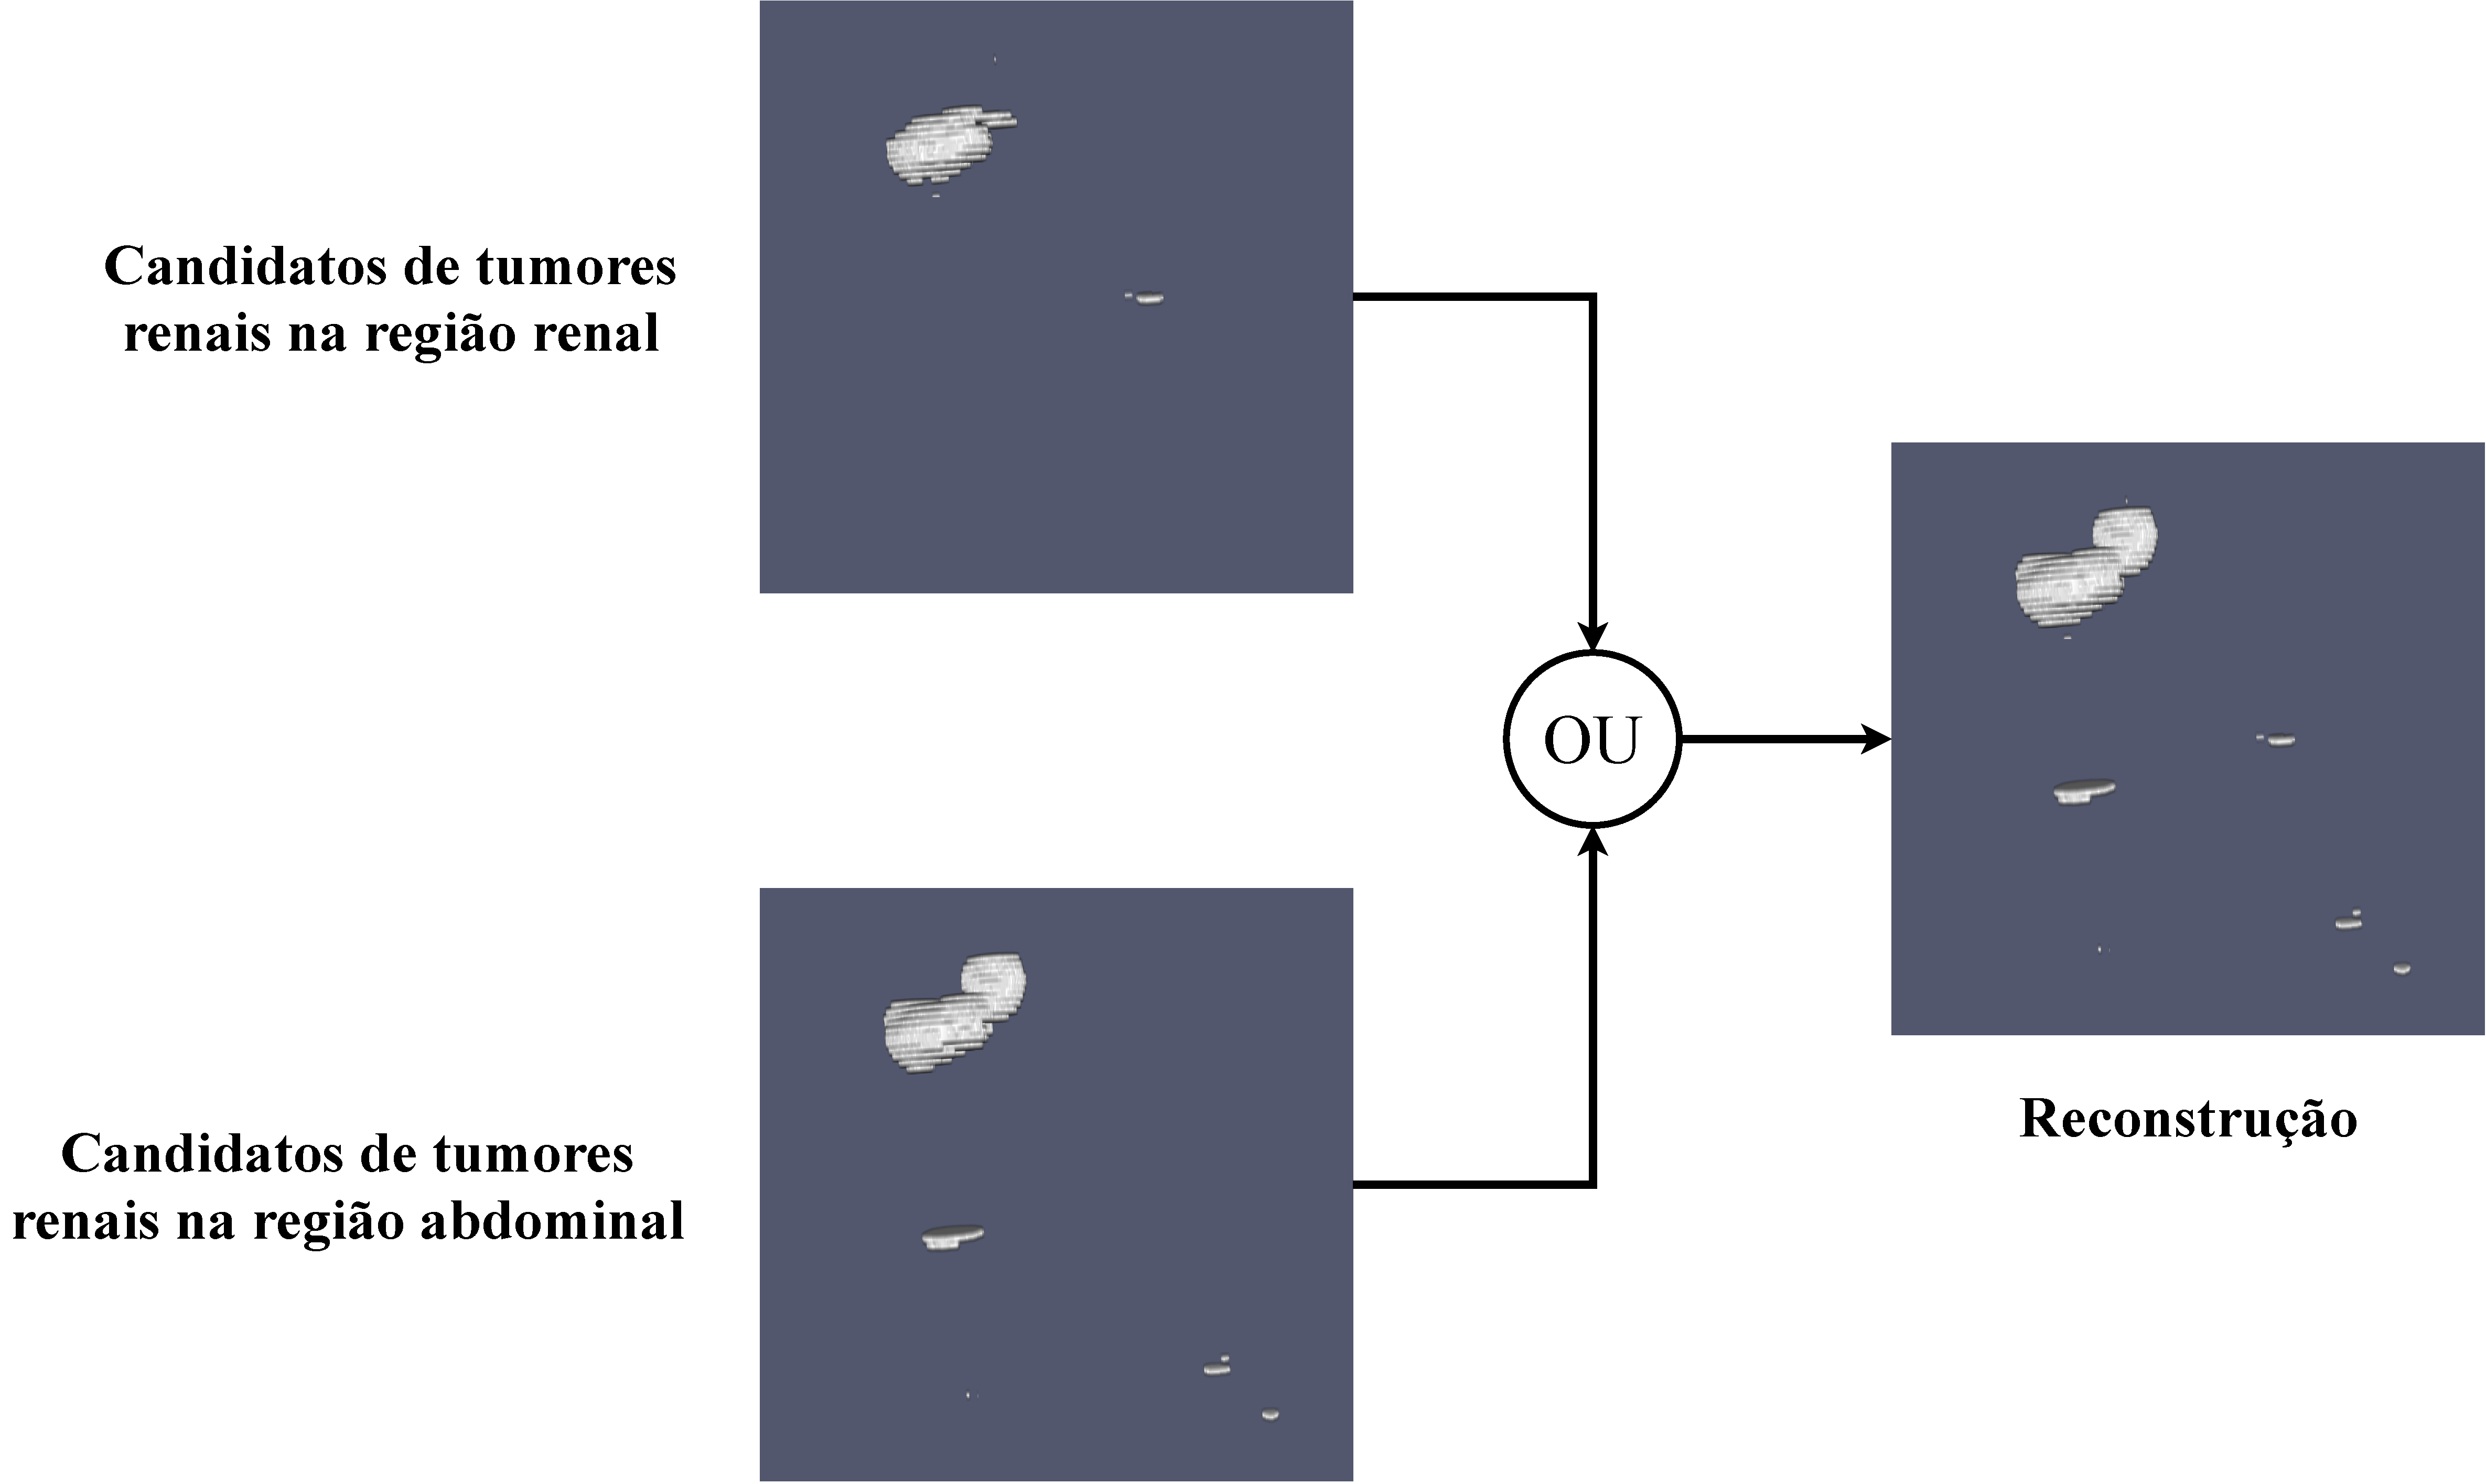
\includegraphics[width=0.9\textwidth]{figuras/reconstrucao.pdf}
    \legend{Fonte: Elaborado pela autora.}
    \label{fig:reconstrucao}
\end{figure}

%O principal benefício da reconstrução é que esta etapa é capaz de recuperar uma porção considerável das regiões tumorais nas quais a diferença de textura o afetou, além de obter uma melhor definição dos contornos tumorais. No entanto, também pode segmentar várias regiões que não são tumores renais. Porém, na etapa final de segmentação, essas regiões segmentadas extras são removidas usando o pós-processamento.

O principal benefício da reconstrução dos tumores renais é que esta etapa é capaz de unir porções consideráveis das regiões tumorais, o que resultou em uma melhor definição dos contornos e regiões tumorais. No entanto, também pode segmentar várias regiões que não são tumores. Porém, na etapa final de segmentação, essas regiões segmentadas extras são removidas usando o pós-processamento.

\section{Redução de Falsos Positivos}
\label{sec:metodo-reducao-falsos-positivos}

Nesta etapa são obtidos os resultados finais das segmentações dos rins e tumores. Para isso, o resultado da etapa de reconstrução dos tumores renais é fundamental para se obter o resultado final dos rins e tumores. Mais detalhes são fornecidos nas próximas subseções.

\subsection{Redução de Falsos Positivos para os Rins}
\label{sec:metodo-reducao-falsos-positivos-rins}

Para obter a segmentação final dos rins, foi feito inicialmente uma união da segmentação inicial dos rins com o resultado da etapa de reconstrução dos tumores renais, usando a operação binária “OU” (Figura~\ref{fig:uniao-rins-recons}). O objetivo é melhorar os contornos que não foram obtidos na etapa de segmentação inicial dos rins por meio da reconstrução dos tumores renais, uma vez que os tumores renais também fazem parte da região renal.

\begin{figure}[!ht]
    \centering
    \caption{União da segmentação inicial dos rins e reconstrução dos tumores renais.}
    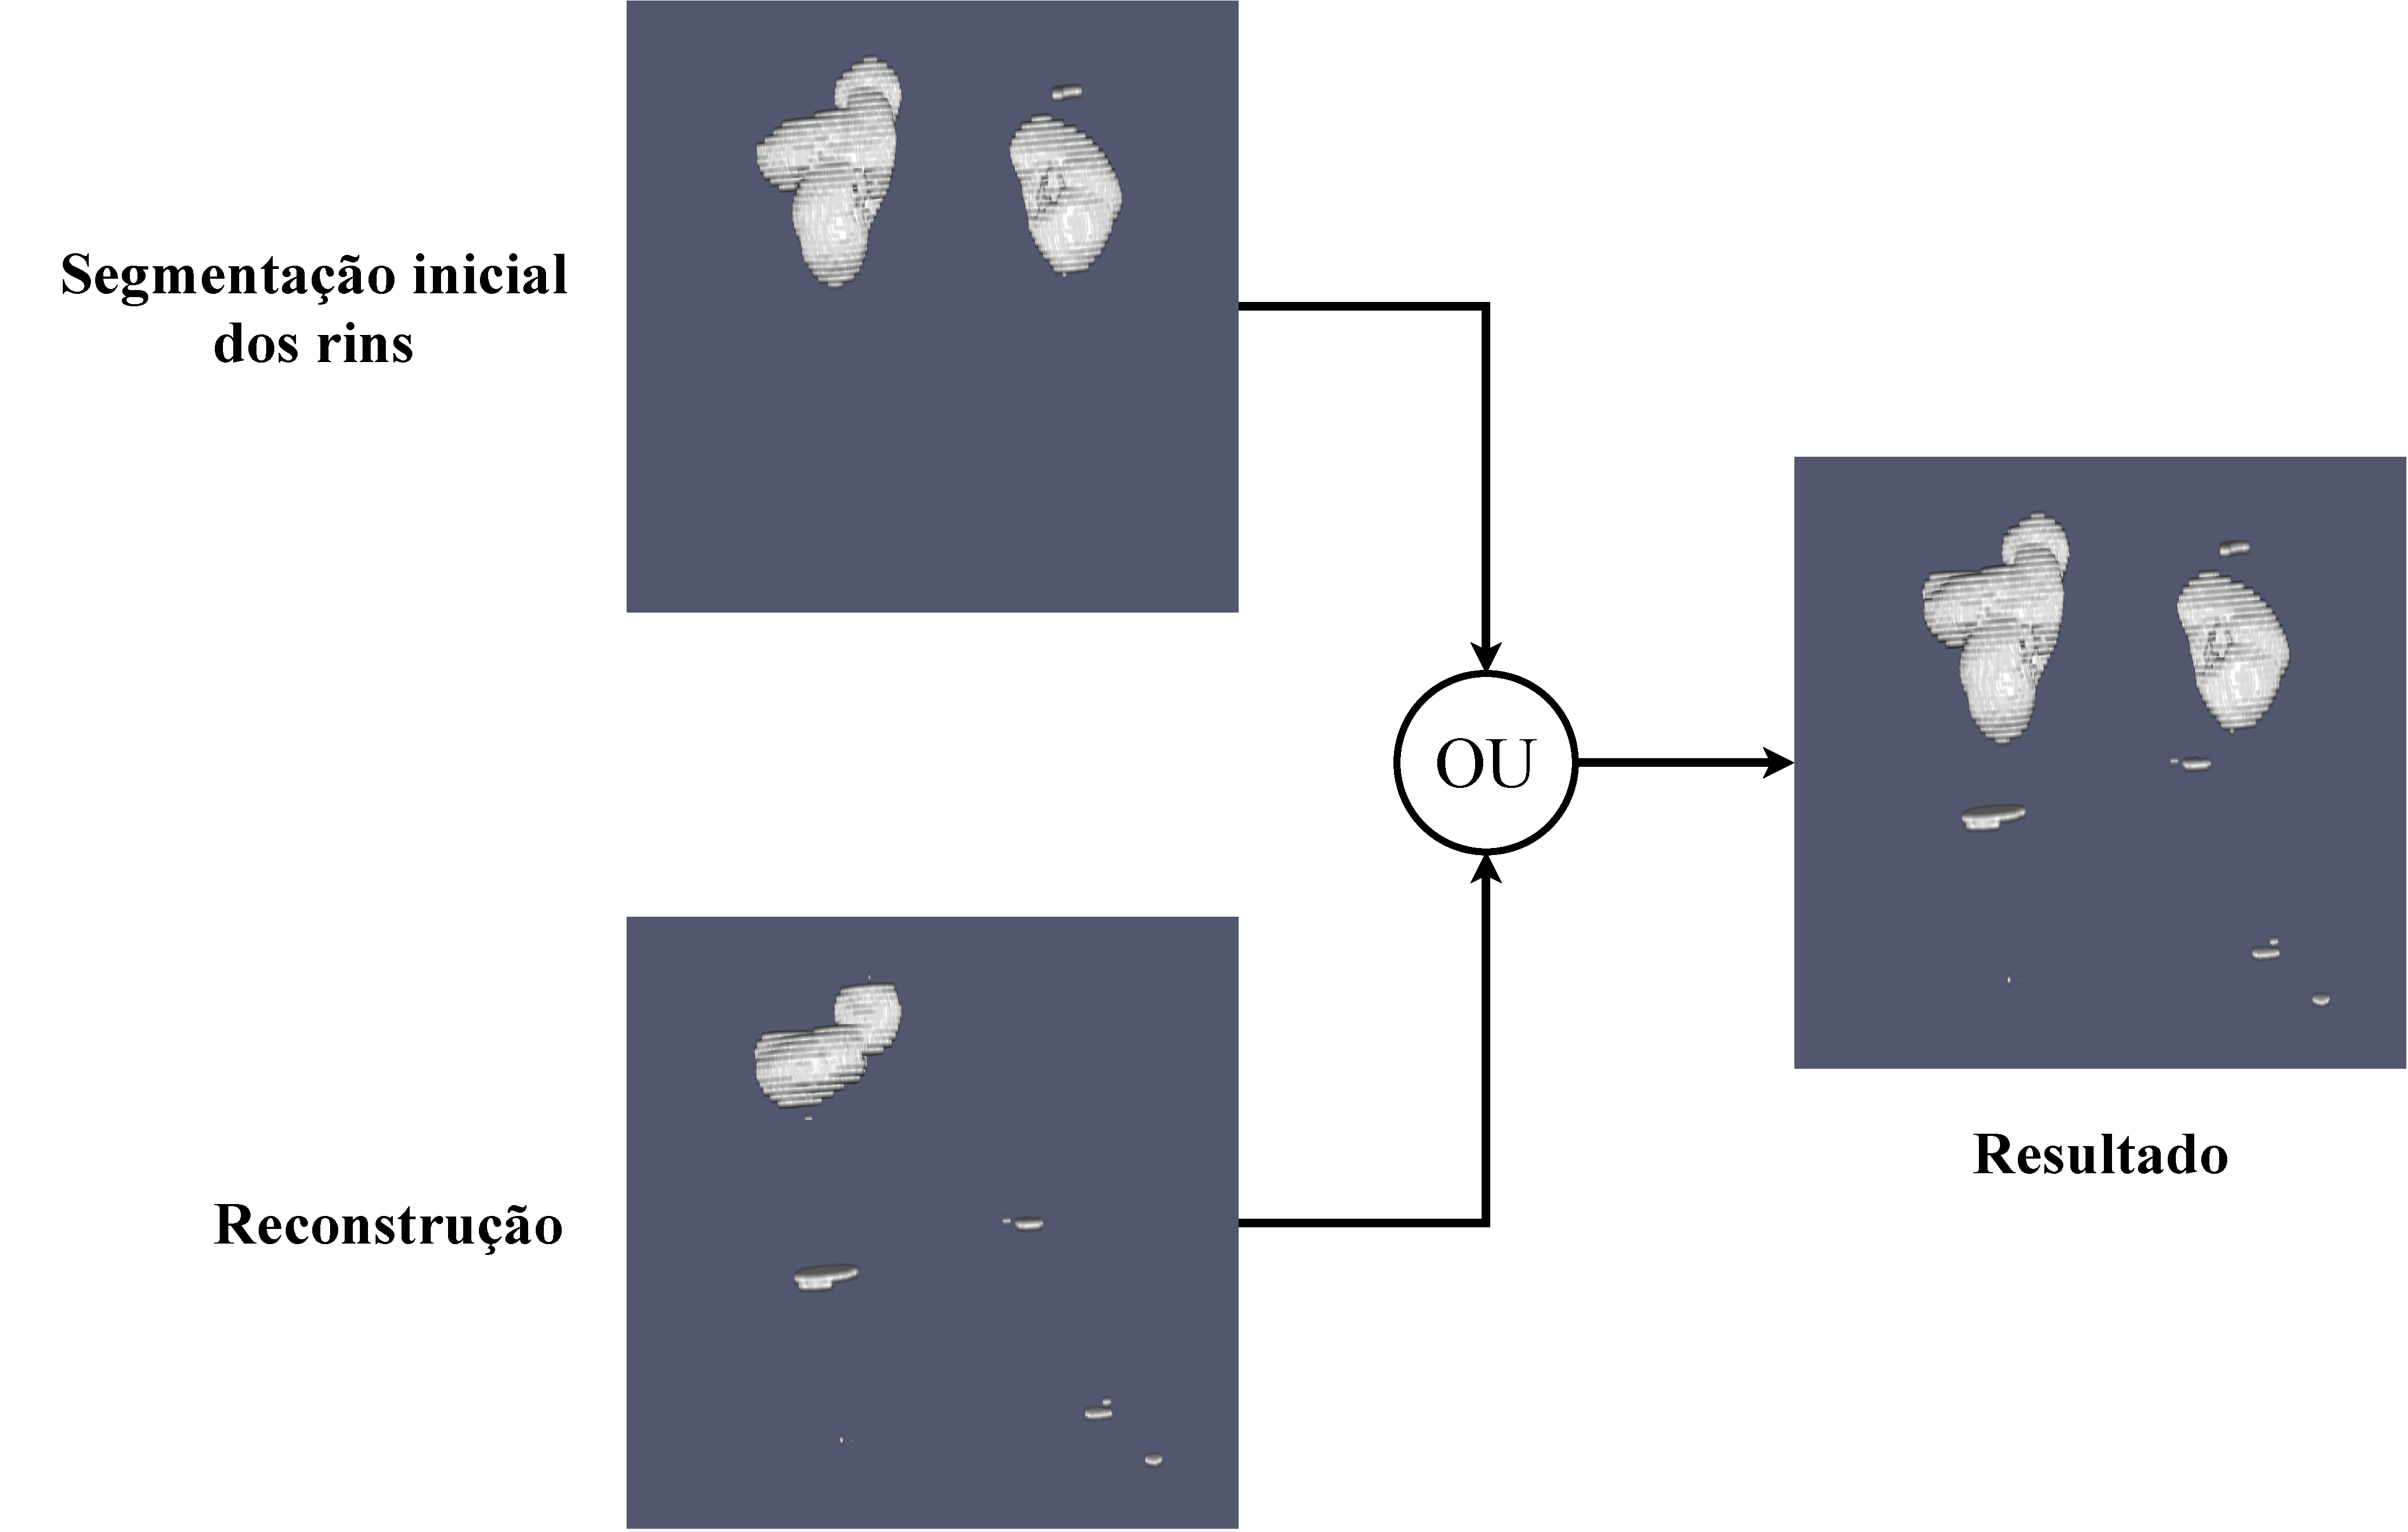
\includegraphics[width=0.9\textwidth]{figuras/uniao-rim-reconstrucao.pdf}
    \legend{Fonte: Elaborado pela autora.}
    \label{fig:uniao-rins-recons}
\end{figure}

No entanto, isso também pode afetar a segmentação inicial dos rins. Portanto, uma etapa de pós-processamento é necessária para remover as regiões que não fazem parte dos rins que foram segmentadas na etapa de união descrita anteriormente. Essa etapa consiste em manter os dois maiores elementos do volume que corresponde aos rins e remover o restante dos fragmentos segmentados (falsos positivos). A Figura~\ref{fig:seg-final-rins}~(a) mostra o resultado em 3D da união descrita anteriormente e a Figura~\ref{fig:seg-final-rins}~(b) a marcação do especialista. Na Figura~\ref{fig:seg-final-rins}~(c) encontra-se o resultado visual após a etapa de pós-processamento. Pode-se observar que alguns fragmentos não renais foram removidos e, consequentemente, a precisão da segmentação dos rins também aumentou.

\begin{figure}[!ht]
    \centering
    \caption{Resultado final da segmentação de rins após pós-processamento.}
    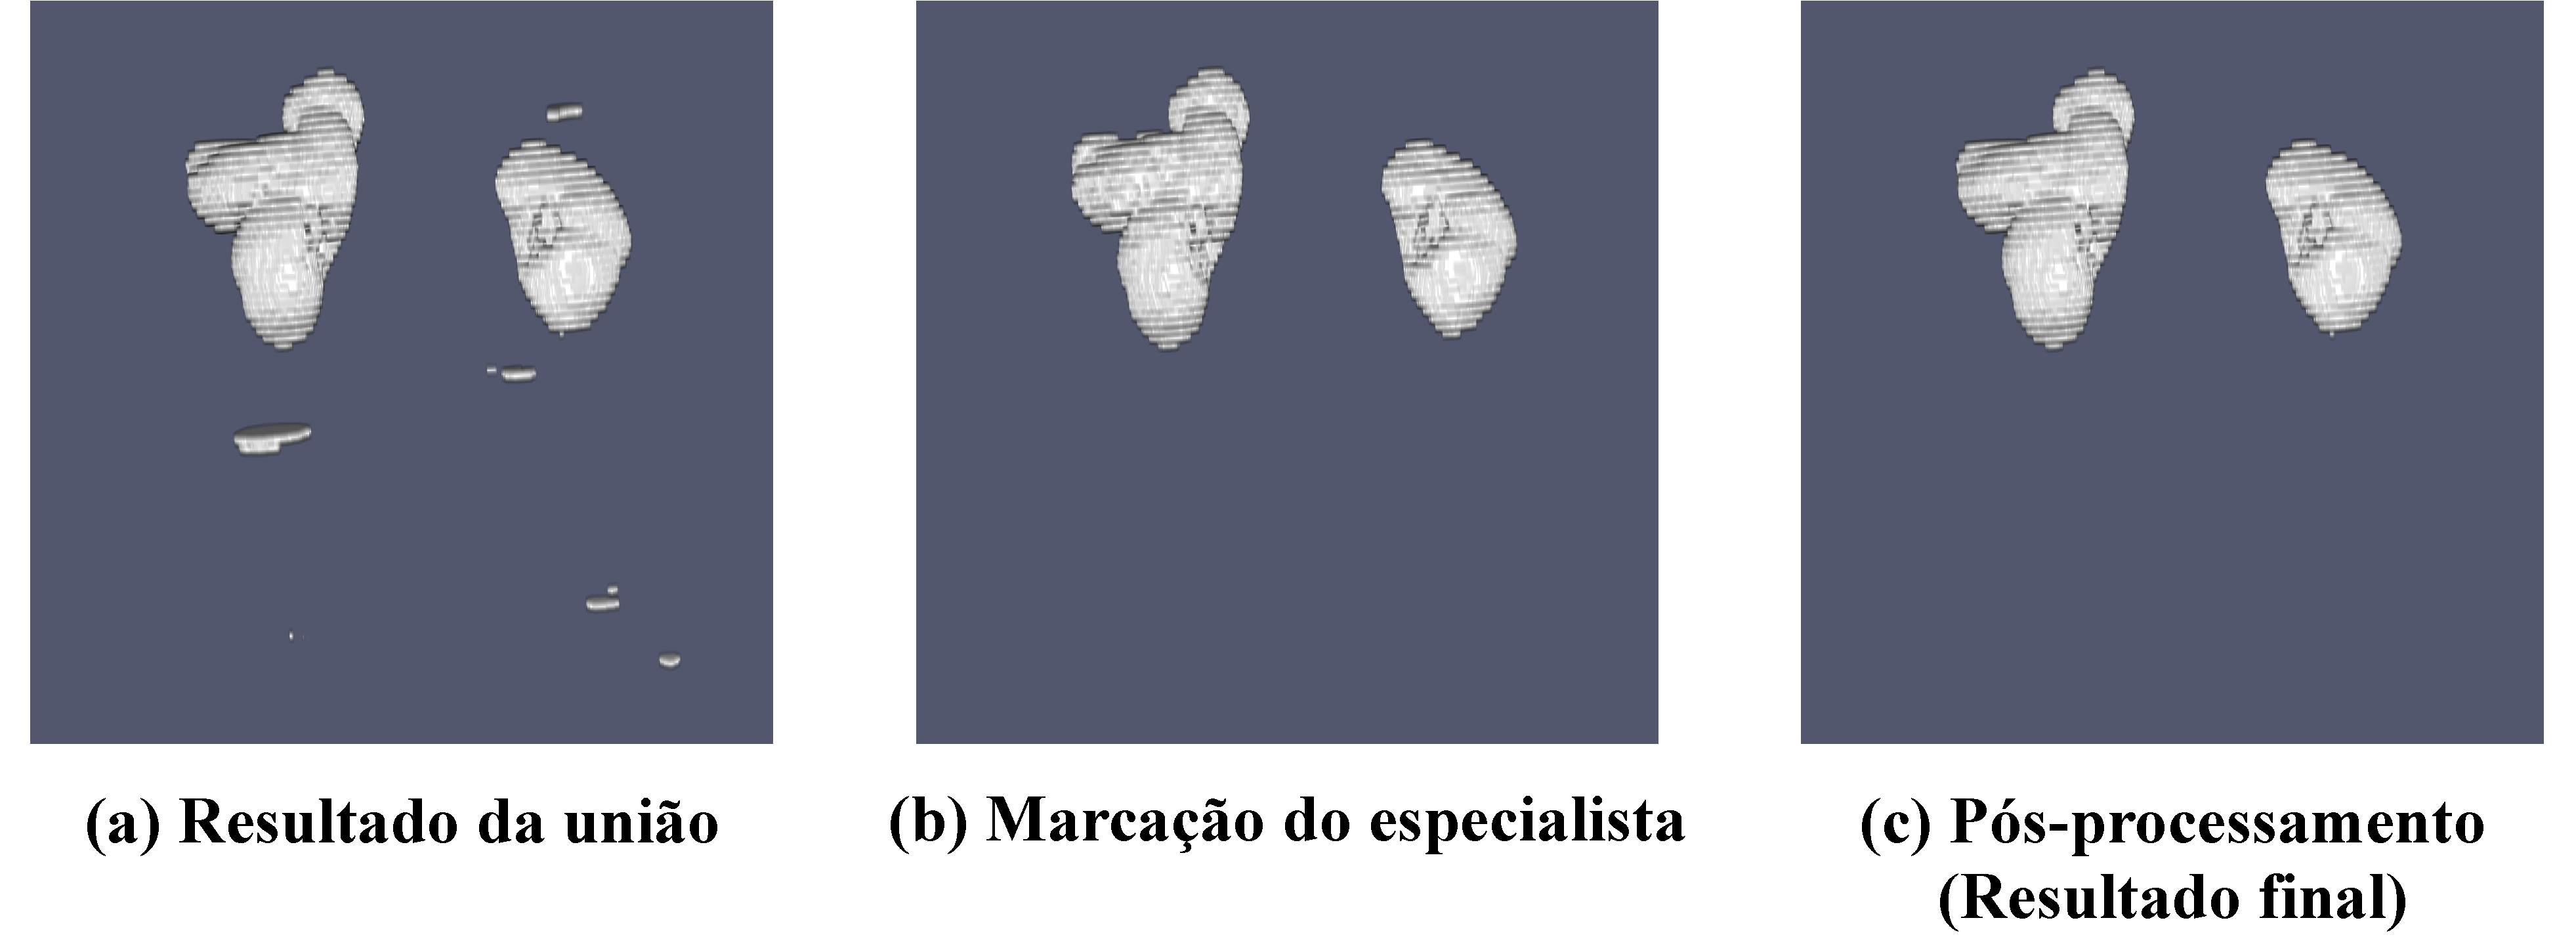
\includegraphics[width=0.9\textwidth]{figuras/rim-final.pdf}
    \legend{Fonte: Elaborado pela autora.}
    \label{fig:seg-final-rins}
\end{figure}

\subsection{Redução de Falsos Positivos para os Tumores Renais}
\label{sec:metodo-reducao-falsos-positivos-tumores-renais}

Nesta subseção são apresentados os procedimentos para obtenção da segmentação final dos tumores renais. Inicialmente, foi aplicada a operação binária “E” para fazer a intersecção da segmentação final dos rins com a etapa de reconstrução dos tumores renais (Figura~\ref{fig:interseccao-rins-recons}). Essa etapa inicial foi feita para extrair apenas a região que contém os tumores, removendo assim parte dos falsos positivos que foram adquiridos na etapa de reconstrução dos tumores renais. Posteriormente, uma etapa de pós-processamento foi aplicada para remover alguns elementos descontínuos que possivelmente eram falsos positivos que permaneceram.

\begin{figure}[!ht]
    \centering
    \caption{Intersecção da segmentação final dos rins e reconstrução dos tumores renais.}
    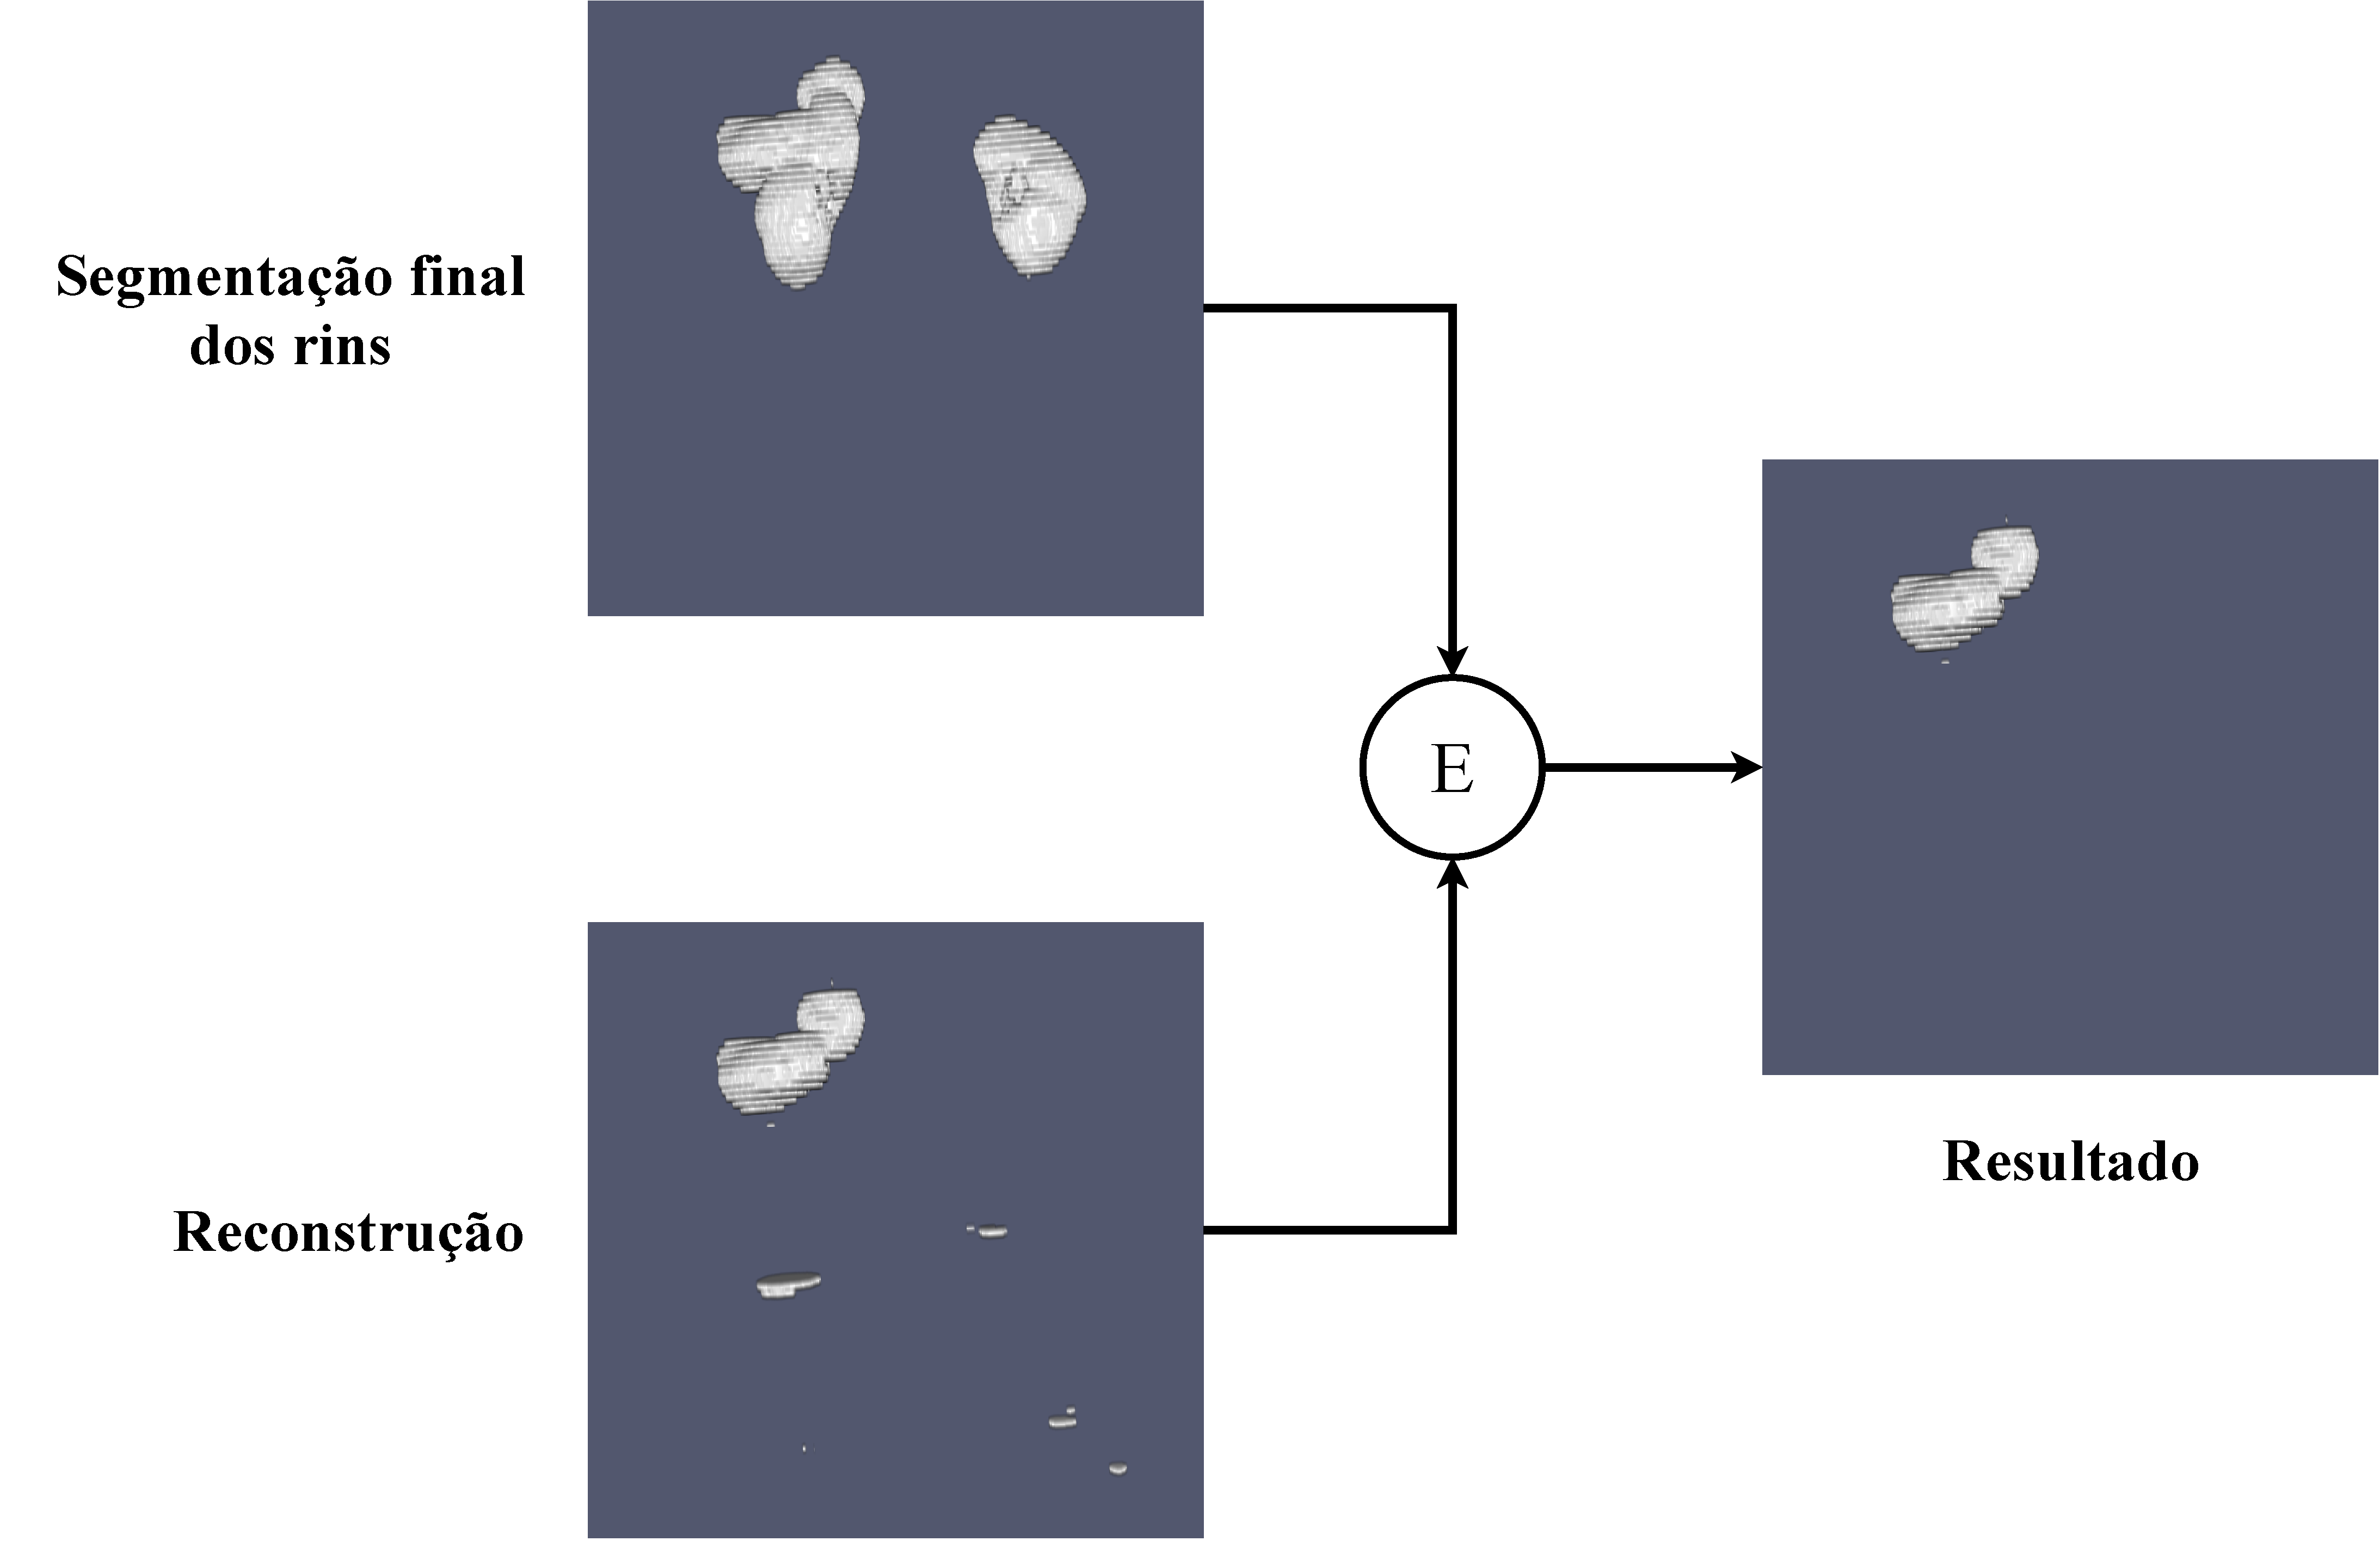
\includegraphics[width=0.9\textwidth]{figuras/interseccao-rim-reconstrucao.pdf}
    \legend{Fonte: Elaborado pela autora.}
    \label{fig:interseccao-rins-recons}
\end{figure}

Os tumores renais são estruturas contínuas que aparecem em várias fatias de um volume de TC~\cite{urology_health,urology_care}. Analisando as informações contextuais vizinhas, o modelo DeepLabv3+ 2.5D resultou na segmentação da fatia central. Portanto, é fundamental verificar se os elementos segmentados pertencem à mesma região. Assim, a etapa de pós-processamento desenvolvida remove as estruturas segmentadas sem informações contextuais suficientes para representar os tumores renais, ou seja, elementos que apresentavam menos de três fatias contínuas.

A Figura~\ref{fig:seg-final-tumores} ilustra a etapa de pós-processamento aplicada. Na Figura~\ref{fig:seg-final-tumores} (a), tem-se o resultado em 3D da interseção descrita acima e a Figura~\ref{fig:seg-final-tumores} (b) mostra a máscara do especialista. Por fim, a Figura~\ref{fig:seg-final-tumores} (c) apresenta o resultado visual após a remoção de elementos descontínuos. É possível verificar que alguns falsos positivos restantes semelhantes aos tumores foram removidos. Assim, a etapa de pós-processamento foi capaz de melhorar a segmentação dos tumores.

\begin{figure}[!ht]
    \centering
    \caption{Resultado final da segmentação de tumores renais após a aplicação do pós-processamento.}
    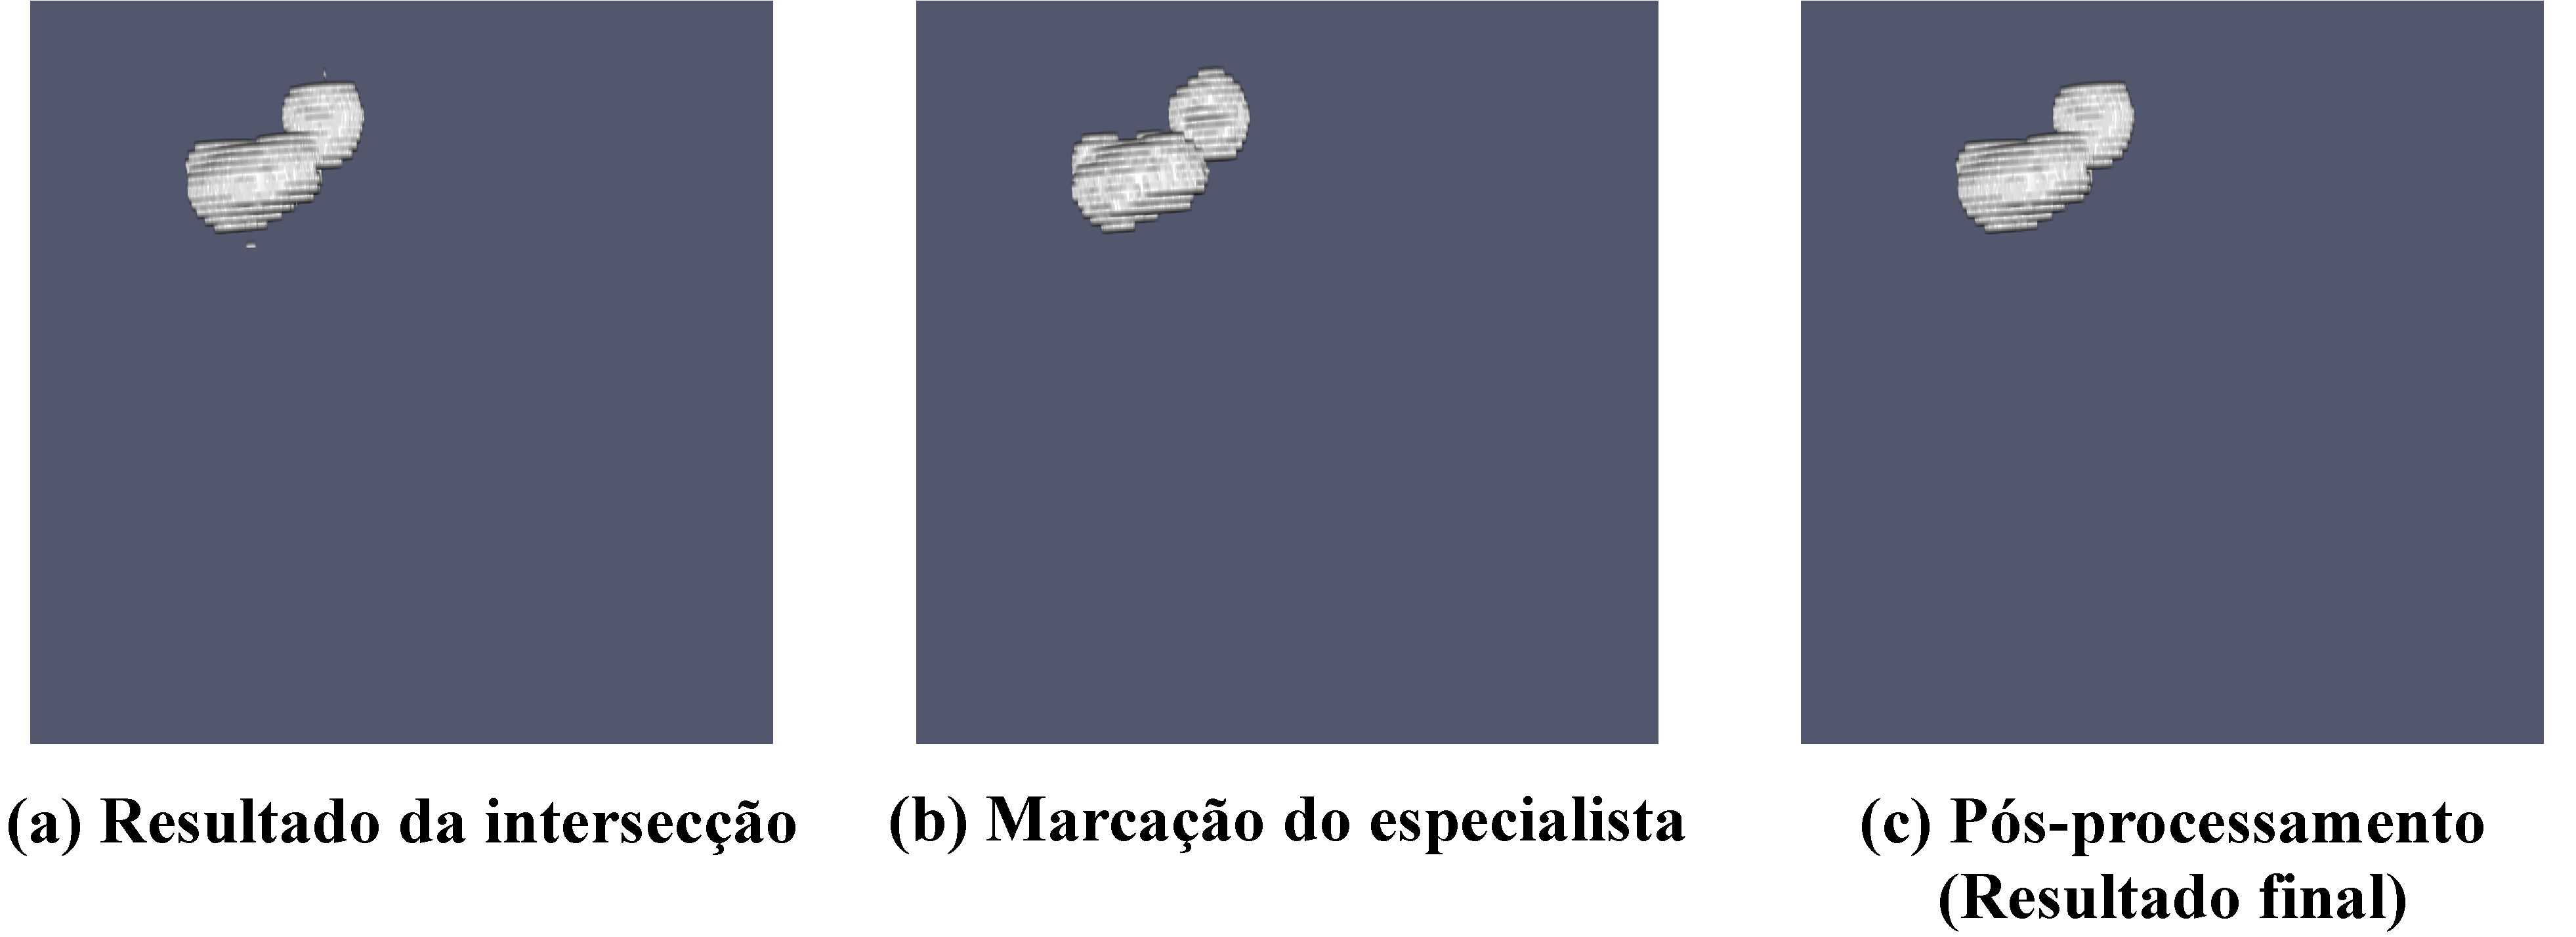
\includegraphics[width=0.9\textwidth]{figuras/tumor-final.pdf}
    \legend{Fonte: Elaborado pela autora.}
    \label{fig:seg-final-tumores}
\end{figure}

\section{Considerações Finais}
\label{consideracoes-finais-metodo}

Este capítulo apresentou e descreveu em detalhes o método proposto para segmentação de rins e tumores em imagens de TC. Foram detalhadas cada uma das etapas que compõem o método, e apresentadas as adaptações empregadas para a segmentação de rins e tumores nesta tese. Entre as principais contribuições estão: a distribuição proporcional da base de imagens; balanceamento de fatias do alvo de segmentação; segmentação de rins e candidatos a tumores renais na região abdominal usando o modelo ResUNet 2.5D; combinação do modelo DeepLabv3+ com o codificador DPN-131 para segmentação de candidatos a tumores renais na região renal; reconstrução dos tumores renais usando operações binárias; e técnicas de processamento de imagens para redução de falsos positivos com base em informações contextuais.

%No próximo capítulo, serão apresentados os resultados com a aplicação do método proposto. Será feita uma discussão acerca dos resultados obtidos, e também uma comparação com os trabalhos descritos na literatura, visando contextualizar a relevância da pesquisa desenvolvida neste trabalho.

No próximo capítulo, serão apresentados os resultados obtidos em cada uma das etapas do método proposto. Além disso, são apresentadas a base de imagens aplicada, a configuração experimental das redes usadas e alguns experimentos para validar as etapas do método proposto.
